
\section{Data and Methods}

  \subsection{Ozonesonde record in the Southern Ocean}
  \label{Section:ozonesondes}
    %(Too basic)Ozonesondes are weather balloons which measure ozone concentrations from the surface to around 35km.
    %These ozonesondes provide a high vertical resolution profile of ozone, along with temperature, pressure, and humidity.
    Ozonesondes provide a high vertical resolution profile of ozone, temperature, pressure, and humidity from the surface to 35 km.
    In the troposphere (up to roughly 10~km) the ozonesondes generally take 150-300 measurements.
    
    Ozone mixing ratio is quantified with an electrochemical concentration cell that senses the proportional electrical current from reaction of ozone with a solution of potassium iodide.
    %(relevance) Most ozonesondes are new and independant, since retrieval of a used ozonesonde can be difficult.
    Standardised procedures are followed when constructing, transporting, and releasing the ozonesondes \citep{noaasondes}.
    Ozonesondes are estimated to provide around 2\% precision in the stratosphere, which improves at lower altitudes \citep{noaasondes}, and ozonesondes have been shown to be accurate to within 5\% when the correct procedures are followed \citep{Smit2007}.
    
    Ozonesondes are launched approximately weekly from Melbourne (38$^{\circ}$ S, 145$^{\circ}$ E), Macquarie Island (55$^{\circ}$ S, 159$^{\circ}$ E) and Davis (69$^{\circ}$ S, 78$^{\circ}$ E). 
    For this study, we use the data collected from 2004-2013 for Melbourne and Macquarie, and 2006-2013 for Davis because both ozone and geopotential height (GPH) profiles were measured during these periods.
    At Davis, ozonesondes are launched twice as frequently during the ozone hole season and preceding months (June-October) as at other times of year \citep{Alexander2013}.
    A summary of ozonesondes at each site can be seen in Table \ref{table:sondesummary}.
    
    \begin{table}[t]
      %\centering
      \caption{Seasonal distribution of sonde releases per site.}
      \begin{tabular}{| c | c | c | c |} 
	\hline
	Site & Sondes & Monthly (JFMAM...) & Date Range \\
	\hline
	Davis     & 240 & 11, 12, 13, 12, 17, 31,	& 2006/04/13 -  \\ 
		  &	& 29, 28, 32, 28, 15, 12 	& 2013/11/13	\\
	Macquarie & 390 & 32, 31, 45, 28, 34, 33,	& 2004/01/20 -  \\
		  &	& 28, 35, 29, 33, 31, 31 	& 2013/01/09	\\ 
	Melbourne & 456 & 31, 38, 40, 38, 41, 36,	& 2004/01/08 -  \\
		  &	& 38, 39, 46, 40, 38, 31        & 2013/12/18	\\
	\hline
      \end{tabular}
      \label{table:sondesummary}
    \end{table}
    
    Characterisation of STT events requires a clear definition of the tropopause.
    The two most common tropopause height definitions are the standard lapse rate tropopause \citep{WMO1957} and the ozone tropopause \citep{Bethan1996}.
    The lapse rate tropopause is defined as the lowest altitude where the lapse rate (vertical gradient of temperature) is less than 2$^\circ$C~km$^{-1}$, provided the lapse rate between this altitude and 2~km above is also below 2$^\circ$C~km$^{-1}$.
    The ozone tropopause is defined as the lowest altitude satisfying the following three conditions for the ozone mixing ratio (OMR) \citep{Bethan1996}:
    \begin{enumerate}
      \item Vertical gradient of OMR is greater than 60~ppb km$^{-1}$;
      \item OMR is greater than 80~ppb; and
      \item OMR exceeds 110~ppb between 500~m and 2000~m above the altitude under inspection (500~m and 1500~m in the Antarctic, including the site at Davis).
    \end{enumerate}
    The ozone tropopause can be less robust during stratosphere-troposphere exchange; however, it is more robust than the lapse rate tropopause at polar latitudes in winter and near jet streams in the lower stratosphere due to temperature inversions near the tropopause \citep{Bethan1996, Tomikawa2009, Alexander2013}.
    In this work, the lower of these two tropopause altitudes is used. 
    This choice avoids occasional unrealistically high tropopause heights due to perturbed ozone or temperature measurements in the ozonesonde data.
    
    Figure \ref{fig:seasonaltpheights} shows the monthly mean tropopause altitudes at each location (solid lines).
    At Melbourne, tropopause altitude displays a seasonal cycle with maximum in summer and minimum is winter.
    This seasonality is missing at Macquarie and almost reversed at Davis, which has a minimum during autumn and maximum from winter to spring.
    Tropopause altitude decreases with latitude from 9-12 km at Melbourne (38$^\circ$S) to 7-9 km at Davis (69$^\circ$S).
    %The tropopause is higher on days with an STT event at all during winter and spring at Davis.

    \begin{figure}[t] 
    % figure produced in seasonal_tropopause in Examine_stations.py
      %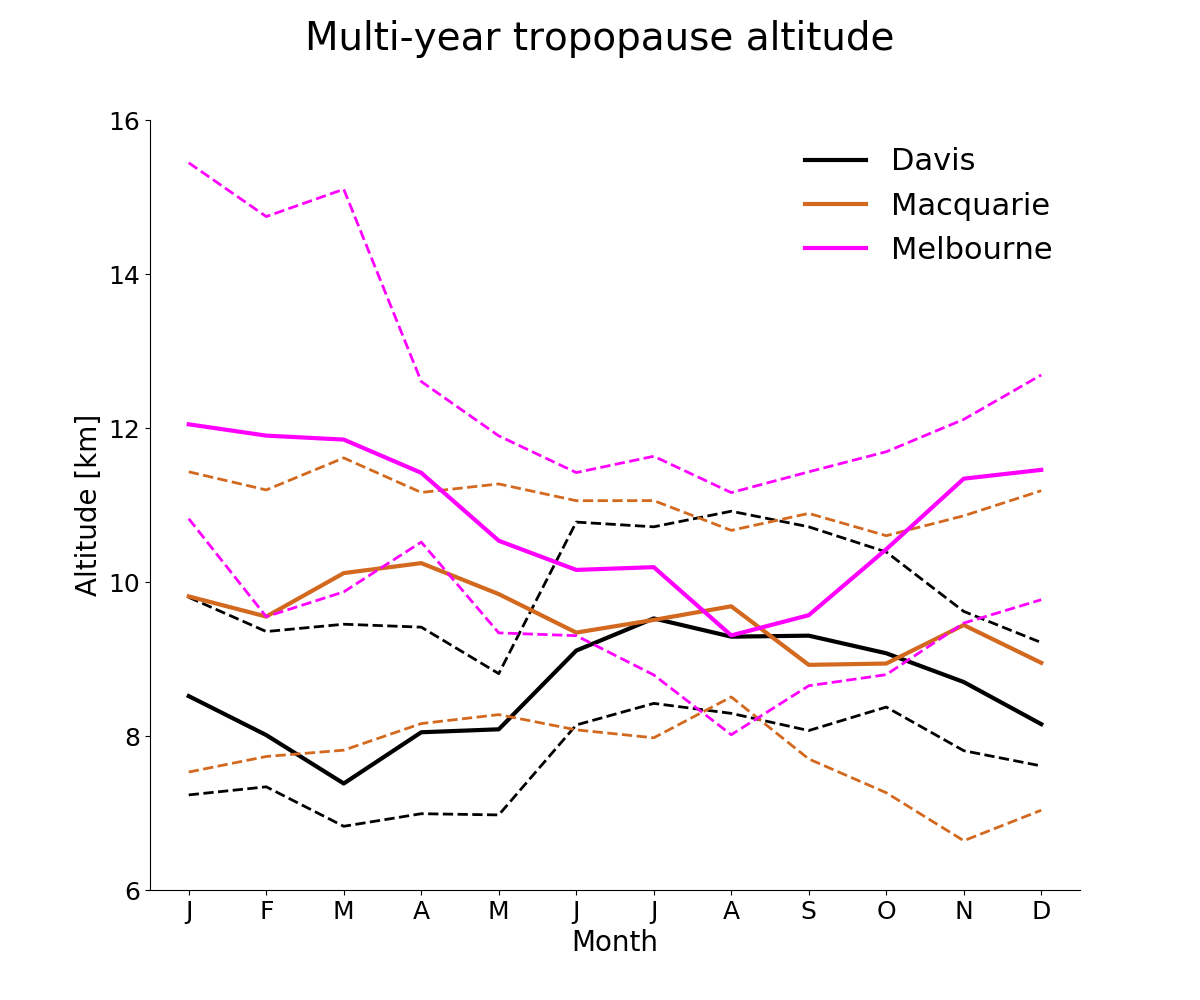
\includegraphics[width=0.8\columnwidth]{figures/tpheights}
      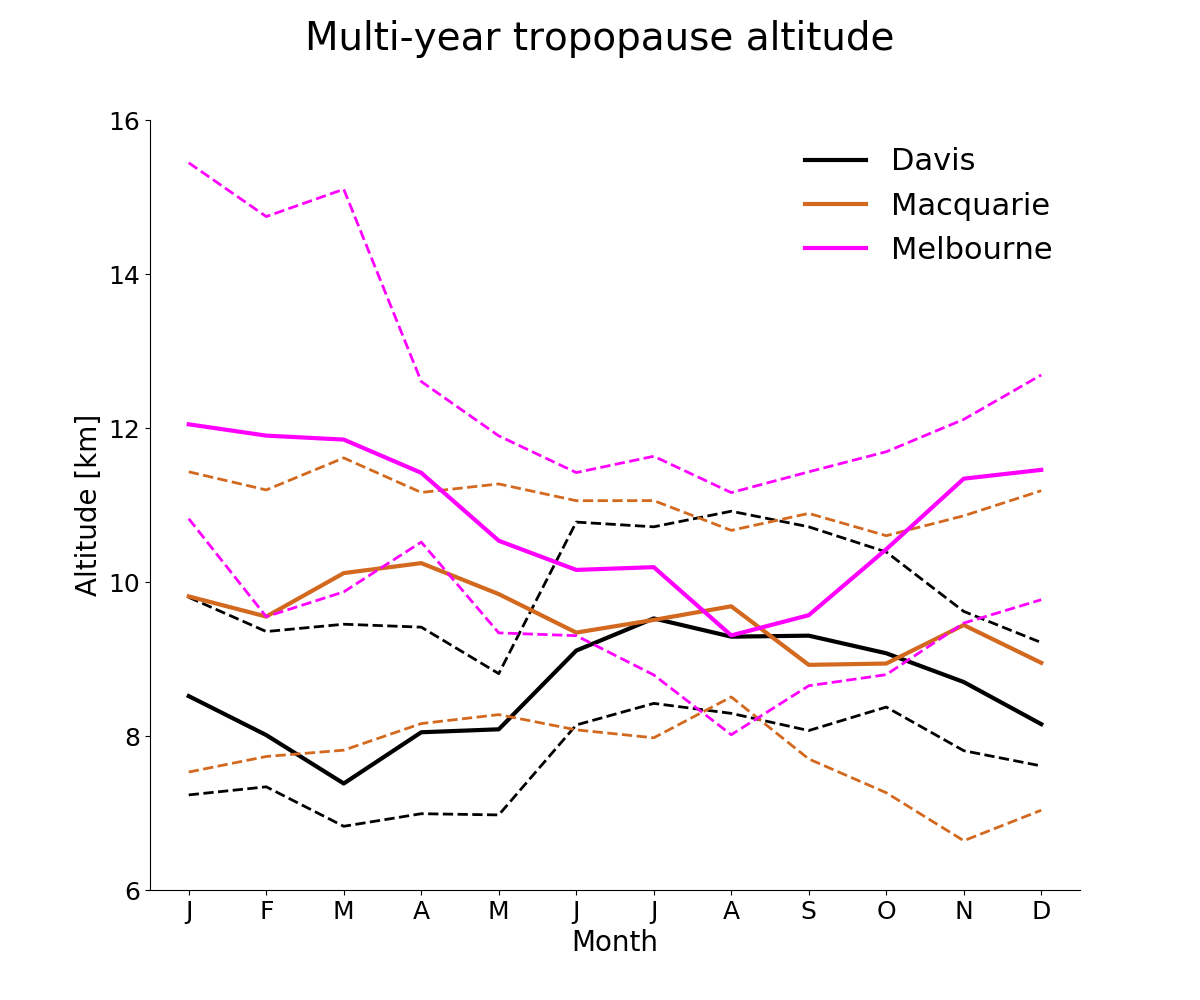
\includegraphics[width=8.3cm]{figures/tpheights}
      \caption{%
	Multi-year monthly median tropopause altitude (minimum of lapse rate and ozone defined tropopause) determined from ozonesondes measurements at Melbourne (2004-2013), Macquarie (2004-2013) and Davis (2006-2013) (solid lines).
	Vertical shading shows the 10th to the 90th percentile of tropopause altitude for each site.}
      \label{fig:seasonaltpheights}
    \end{figure}

    Figure \ref{fig:seasonaltropozone} shows multi-year averaged ozone mixing ratios measured by ozonesonde over the three stations.
    Over Melbourne, increased ozone extending down through the troposphere is apparent from December to March and from September to November.
    The increased tropospheric ozone in these months is due to STT (in summer), and possible biomass burning influence (in winter), both discussed in more detail below.
    Over Davis and Macquarie Island, tropospheric ozone is higher between March and October, although the seasonal differences are small compared to those at Melbourne.
    This seasonality at the high latitude sites is driven by a decrease in photochemical destruction under the reduced radiation conditions around polar night. % (TODO: read and cite S. Oltmans antarctic papers - re Andrews comment)... Can't find paper.
    
    \begin{figure*}[t]
      %Figure created seasonal_tropozone function in examine stations - ported from IDL
      %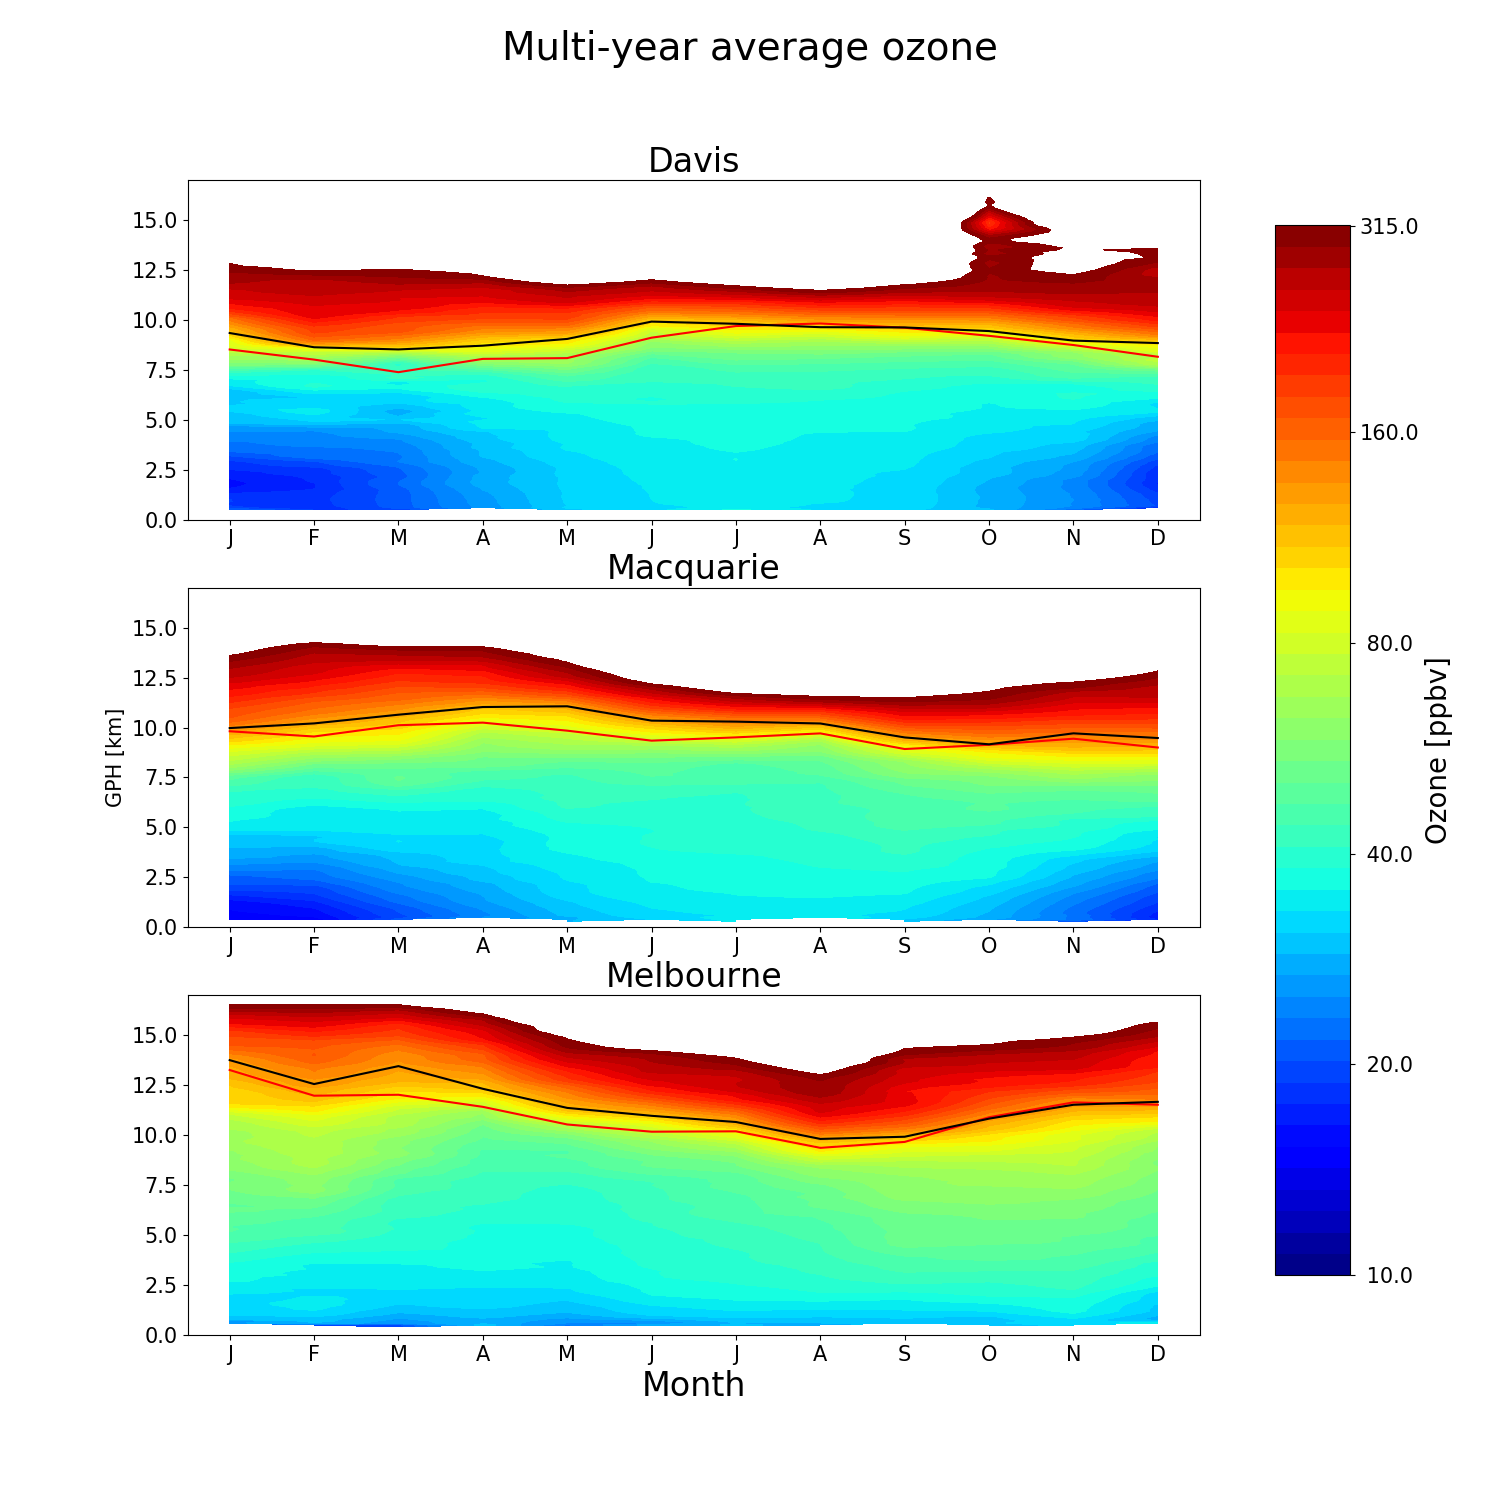
\includegraphics[width=0.95\columnwidth]{figures/seasonaltropozone}
      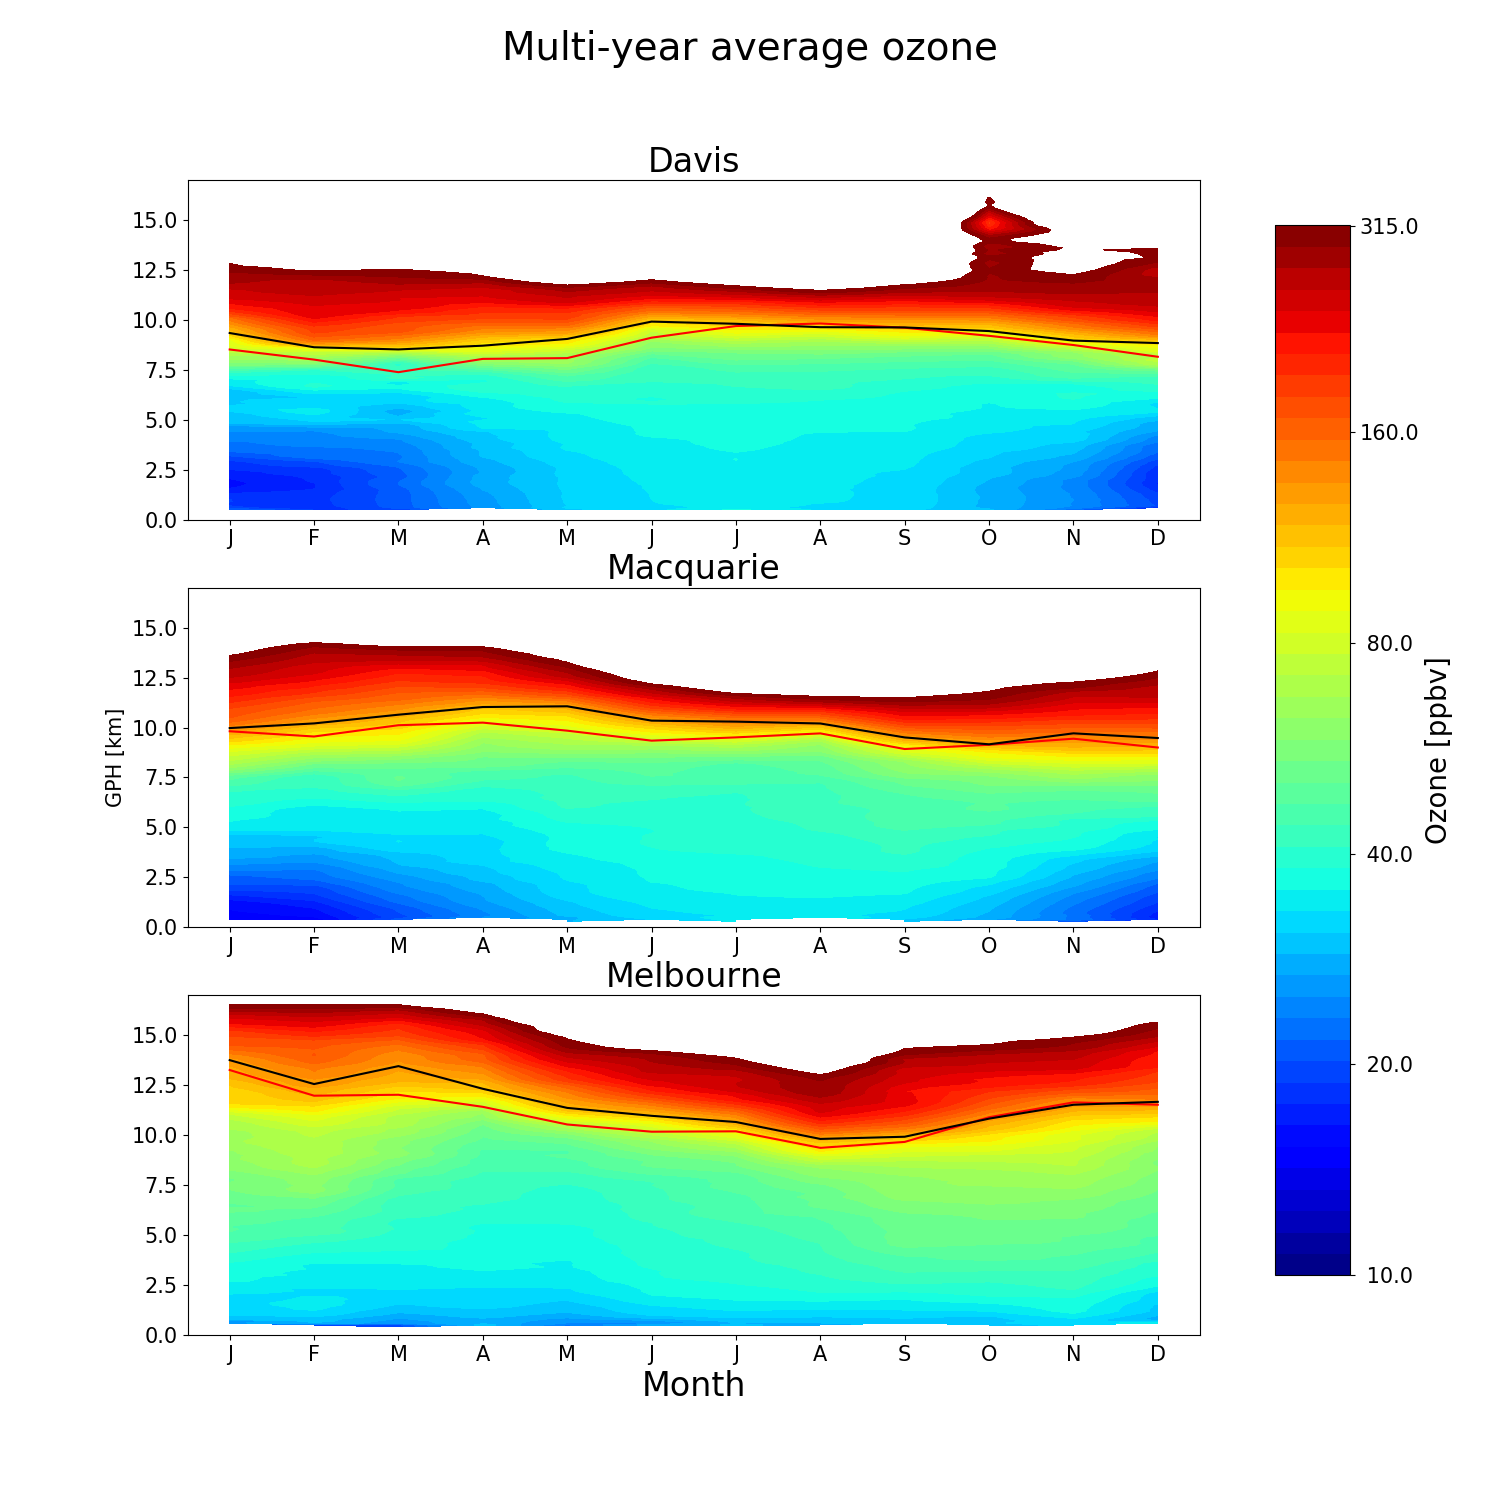
\includegraphics[width=12.0cm]{figures/seasonaltropozone}
      \caption{ %
	Multi-year mean seasonal cycle of ozone mixing ratio over Davis, Macquarie, and Melbourne as measured by ozonesondes.
	Measurements were interpolated to every 100~m and then binned monthly.
	Black and red solid lines show median ozone and lapse-rate defined tropopause altitudes (respectively), defined as described in the text. }
      \label{fig:seasonaltropozone}
    \end{figure*}

  \subsection{Model description}
    \label{Section:GEOSChemDescription}
    To provide regional context to the ozonesonde observations, we use the GEOS-Chem version 10-01 global chemical transport model \citep{Bey2001}, which simulates ozone along with more than 100 other trace gases throughout the troposphere and stratosphere. 
    Stratosphere-troposphere coupling is calculated using the stratospheric unified chemistry extension (UCX) \citep{Eastham2014}.
    Transport is driven by assimilated meteorological fields from the Goddard Earth Observing System (GEOS-5) maintained by the Global Modeling and Assimilation Office (GMAO) at NASA.
    Ozone precursor emissions are from the Model of Emissions of Gases and Aerosols from Nature (MEGAN) version 2.1 \citep{Guenther2012} for biogenic species and from the Emissions Database for Global Atmospheric Research (EDGAR) version 4.2 for anthropogenic species.
    Simulated biomass burning production is driven by the Global Fire Emissions Database (GFED4) inventory \citep{Giglio2013}. 
    Our simulation was modified from the standard v10-01 to fix a bug in the treatment of Total Ozone Mapping Spectrometer (TOMS) satellite data used to calculate photolysis (see \url{http://wiki.seas.harvard.edu/geos-chem/index.php/FAST-JX_v7.0_photolysis_mechanism#Fix_for_TOMS_to_address_strange_cycle_in_OH_output.}).  

    Our simulations span 2005-2012 (following a 1-year spin-up over 2004) with horizontal resolution of 2$^{\circ}$ latitude by 2.5$^{\circ}$ longitude and 72 vertical levels from the surface to 0.01~hPa.
    For comparison to the ozonesonde observations, the model state was saved every 6 hours within the grid boxes containing each site.
    When comparing against ozonesondes, GEOS-Chem UTC+0 time samples are used for all sites.
    This means that the simulated ozone profiles are analysed at local times of 7AM for Davis, and 11AM for Macquarie and Melbourne.
    
  \subsection{Characterisation of STT events and associated fluxes}
    \label{Section:CharacterisationOfSTTs}
    
    We characterise STT events using the ozonesonde vertical profiles to identify tropospheric ozone enhancements above a local background (in moles per billion moles of dry air, referred to here as ppb).
    %Calculation of ozone transport is performed after converting the profile to molecules cm$^{-3}$.
    The process is illustrated in Figure~\ref{fig:filterEG} on an example ozone profile.
    First, the ozone vertical profiles are linearly interpolated to a regular grid with 20~m resolution from the surface to 14~km altitude. 
    The interpolated profiles are then bandpass-filtered using a Fourier transform to retain perturbations with vertical scales between 0.5~km and 5~km (removing low and high frequency perturbations).
    In what follows, these filtered vertical profiles are referred to as perturbation profiles.
    The choice of band limits was set empirically in order to remove the slow positive gradient of ozone over altitude as well as any measurement noise.
    For an event to qualify as STT, a clear increase above the background ozone level is needed, and we find that a bandpass filter removes seasonal-scale effects.
    The 0.5~km scale limit is set in order to remove any spikes of ozone which could be considered noise.
    We next use all the perturbation profiles at each site to calculate the 99th percentile perturbation value for the site.
    This is our threshold for tropospheric ozone perturbations, any profiles with perturbations exceeding this value in individual ozonesondes are classified as STT events.
    STT events at altitudes below 4~km are removed to avoid surface pollution, and events within 0.5~km of the tropopause are removed to avoid false positives induced by the sharp transition to stratospheric air.
    
    \begin{figure}[t]
      % Figure created in getevents.pro, edited in inkscape
      
      %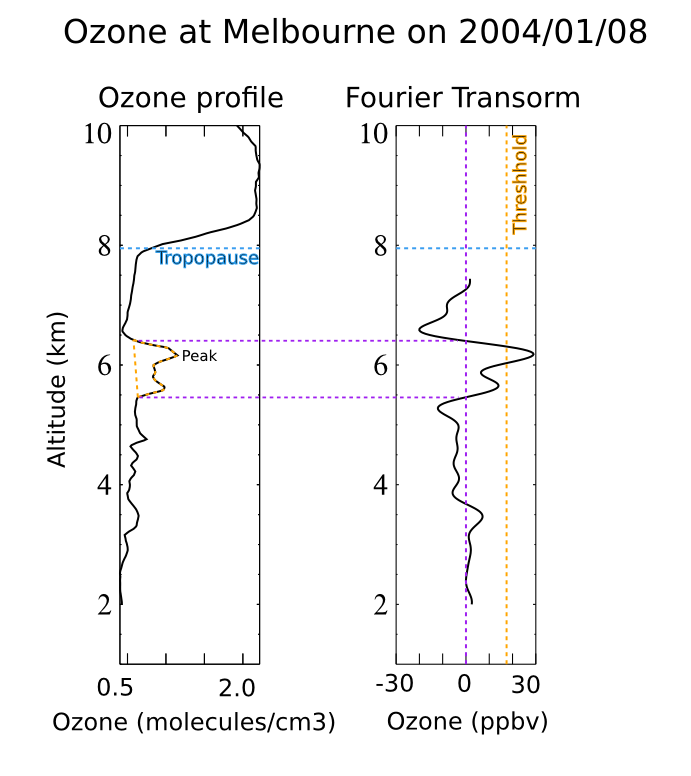
\includegraphics[width=0.8\columnwidth]{figures/filtereg.png}
      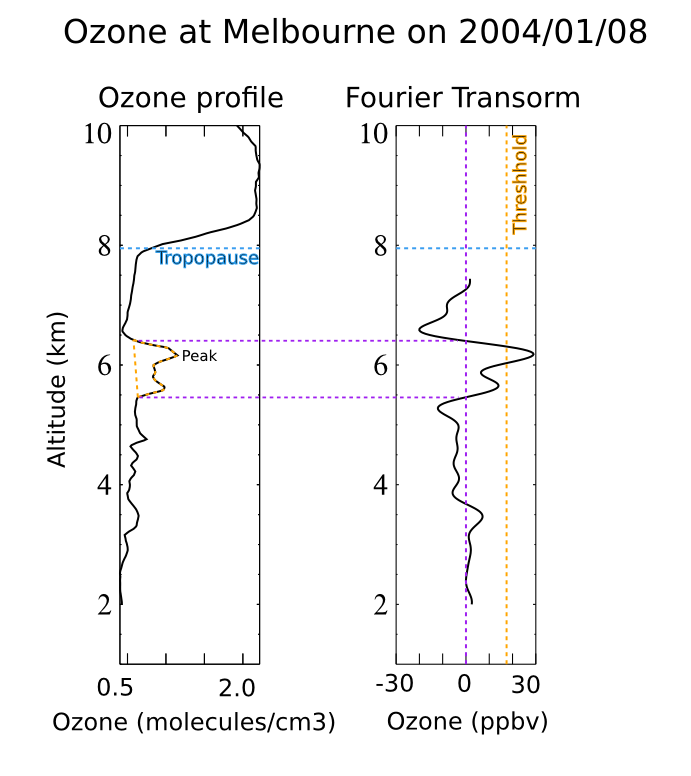
\includegraphics[width=8.3cm]{figures/filtereg.png}
      \caption{ %
	An example of the STT identification and flux estimation methods used in this work. 
	The left panel shows an ozone mixing ratio profile from Melbourne on 8 January 2004 from 2km to the tropopause (dashed horizontal line).
	The right panel shows the perturbation profile created from bandpass filtering of the mixing ratio profile. The STT occurrence threshold calculated from the 99th percentile of all perturbation profiles is shown as the orange dashed line, and the vertical extent of the event is shown with the purple dashed lines (see details in text).
	The ozone flux associated with the STT event is calculated using the area outlined with the orange dashed line in the left panel.
      }
      \label{fig:filterEG}
      
    \end{figure}
   
       
    We define the ozone peak as the altitude where the OMR is greatest within the lowest range of altitudes over which the perturbation profile exceeds the percentile-based threshold.
    The STT event is confirmed if the perturbation profile drops below zero between the ozone peak and the tropopause. 
    Alternatively, the STT event is also confirmed if the OMR between the ozone peak and the tropopause drops below 80~ppb and is at least 20~ppb lower than the OMR at the ozone peak. 
    If neither of these conditions are met, the profile is rejected as a non-event.
    This final step removes near-tropopause anomalies for which there is insufficient evidence of detachment from the stratosphere.
    Vertical ozone profiles recorded by ozonesondes are highly dependent on the time of launch \citep{Sprenger2003}, and it cannot be guaranteed that detected ozone enhancements are fully separated from the stratosphere, although this method minimises that risk by removing detected events too near the tropopause.

    We estimate the ozone flux into the troposphere associated with each event by integrating the ozone concentration enhancement vertically over the altitude range for which an STT event is identified (i.e. enhancement near the ozone peak over which the perturbation profile is greater than zero).
    This estimate is conservative because it does not take into account any secondary ozone enhancements that may have been caused by the STT, and also ignores any enhanced ozone background amounts from synoptic-scale stratospheric mixing into the troposphere.
    
    Our method differs somewhat from that used by \citet{Tang2010} to detect STT events from ozonesonde measurements. 
    Their definition is based on subjective analysis of sondes released from 20 stations ranging in latitude from 35$^\circ$S to 40$^\circ$N.
    They identify an STT event if, starting from 5~km altitude, ozone exceeds 80~ppb and then within 3~km decreases by 20~ppb or more to a value less than 120~ppb.
    Their technique would miss many events due to lower tropospheric ozone concentrations found in the cleaner southern hemisphere.

  \subsection{Biomass burning influence}
  \label{Section:BiomassBurning}
    The STT detection algorithm described in Sect. \ref{Section:CharacterisationOfSTTs} assumes all mid-upper troposphere ozone perturbations above the 99th percentile are caused by stratospheric intrusions. 
    In some cases, however, these perturbations may in fact reflect ozone production in lofted smoke plumes.
    Biomass burning in southern Africa and South America has previously been shown to have a major influence on atmospheric composition in the vicinity of our measurement sites \citep{Oltmans2001, Gloudemans2006, Edwards2006}, particularly from July to December \citep{Pak2003, Liu2016}.
    %The downwind effects of biomass burning smoke plumes from South America and southern Africa are strongest around August and September, as seen here and in \citet{Liu2016}.
    On occasion, smoke plumes from Australian and Indonesian fires can also reach the mid-high southern latitudes, as seen from satellite measurements of carbon monoxide (CO) discussed below. %from the AIRS (Atmospheric Infrared Sounder) instrument on board the Aqua satellite \citep{AIRS3STD}.
    
    %Ozone precursors include nitrogen oxides ($NO_x = NO + NO_2$) and non methane volatile organic compounds (NMVOCs). % too basic for here..
    Large biomass burning events emit substantial quantities of ozone precursors, some of which are capable of being transported long distances and driving ozone production far from the fire source \citep{Jaffe2012}.
    Ozone production from biomass burning is complex and affected by photochemistry, fuel nitrogen load, and time since emission, among other factors. 
    While ozone production occurs in some biomass burning plumes, this is not always the case; therefore ozone perturbations detected during transported smoke events may or may not be caused by the plume.
    For this reason all detected STT events found near smoke plumes are flagged.
    Calculations do not include flagged events however they are included in summary plots in this work.
    
    %Biomass burning influence in the Southern Hemisphere comes mostly from Southern Africa and South America, however Australian fires from the midlatitudes, and Indonesian fires can also influence the ozonesonde release sites.
    %Transported biomass burning plumes influence the southern mid-latitudes generally between July and December \citep{Pak2003}.
    
    Possible biomass burning influence is identified using satellite observations of CO from the AIRS (Atmospheric Infrared Sounder) instrument on board the Aqua satellite \citep{AIRS3STD}.
    CO is emitted during incomplete combustion and is an effective tracer of long-range transport due to its long lifetime \citep{Edwards2003, Edwards2006}.
    In the Southern Hemisphere, biomass burning is the primary source of CO, making CO a good proxy for fire plumes (eg: \citet{Sinha2004, Mari2008}).
    To identify possible biomass burning influence, AIRS vertical column CO is visually inspected for all dates with detected STT events.
    Smoke plumes are diagnosed over areas with elevated CO columns ($\sim 2 \times 10^{18}$ molecules cm$^{-2}$ or higher), and any sonde-detected STT event that occurs near a smoke plume is flagged.

    Figure \ref{fig:excludedeg} contrasts two days with and without signs of biomass burning influence near the Melbourne site (purple circle).
    On 17 October 2007 (top) elevated CO suggests the site may have been influenced by long-range transport from African and/or South American biomass burning.
    In contrast, on 3 February 2006 (bottom) CO columns across the Southern Hemisphere show no influence from biomass burning.
    All days with detected STT events except one event during which there were no available AIRS data (January 2010) are screened.
    It's determined that biomass burning may have influenced 14 events over Melbourne and 8 events over Macquarie island.
    These events are flagged in the following sections, and are not used in our calculation of total STT flux.
    All of the flagged events except for one (in January at Macquarie Island) occur within the Southern Hemisphere burning season (July to December). % burning season cite? \citep{Pak2003}.
    No events at Davis were seen to be influenced by smoke transport.
    
    \begin{figure}[t]
      %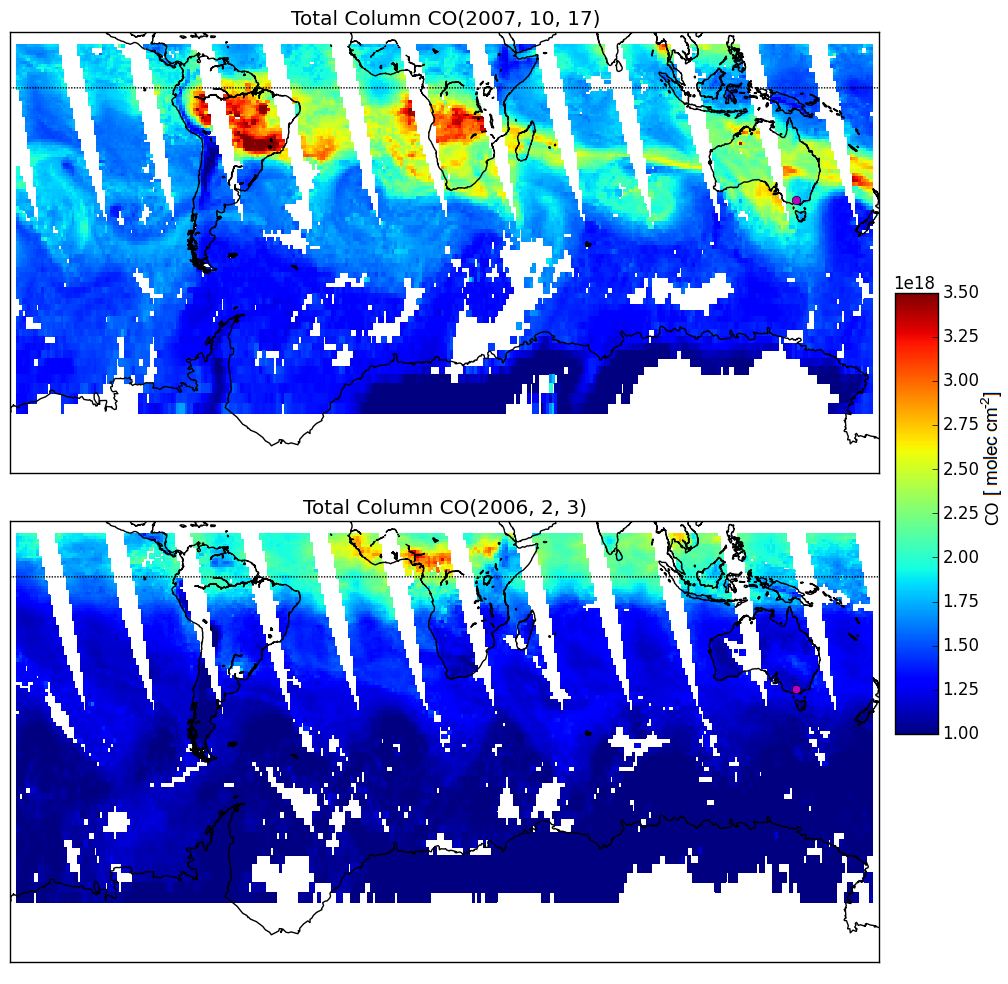
\includegraphics[width=\textwidth]{figures/AIRS_compare.png}
      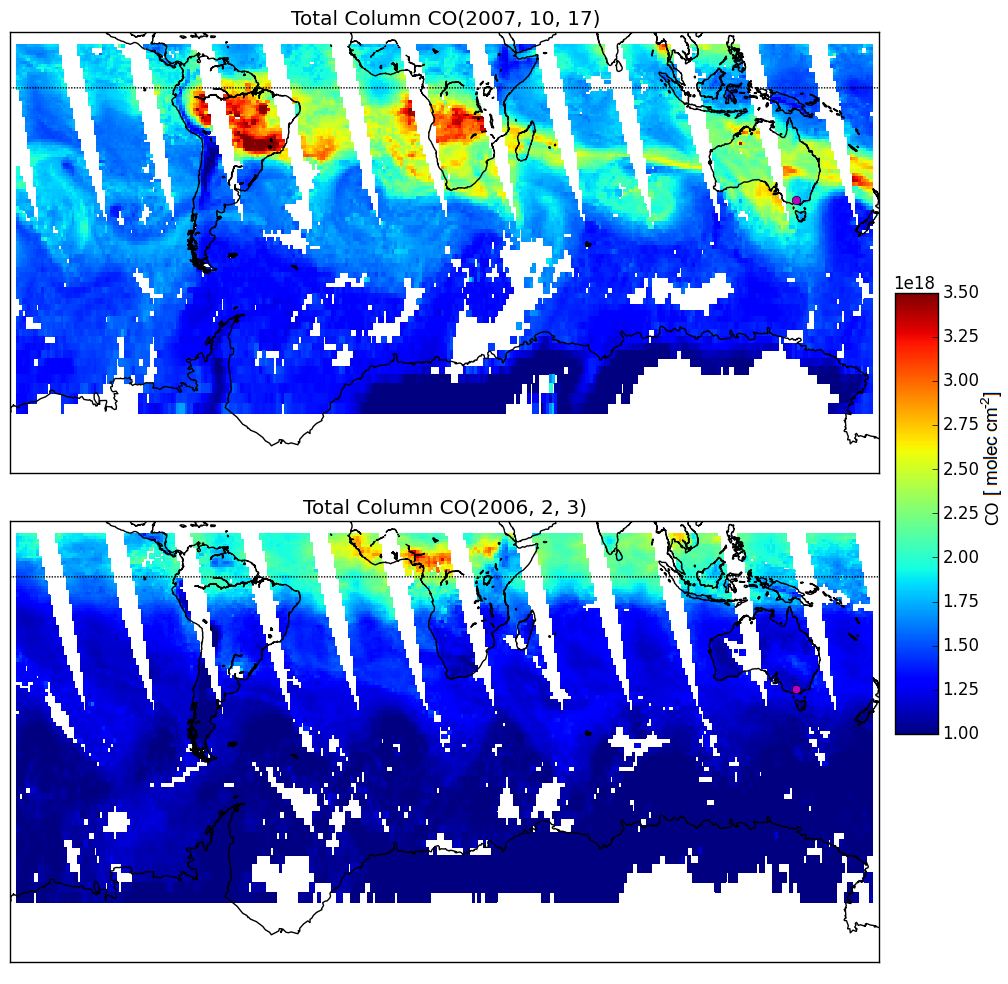
\includegraphics[width=8.3cm]{figures/AIRS_compare.png}
      \caption{ %
	Example detection of biomass burning influence using AIRS total column CO. 
	The top panel (17 October 2007) shows a day when ozone above Melbourne (purple dot) could have been caused by a transported biomass burning plume, and so was flagged in subsequent analysis.
	The bottom panel (3 February 2006) shows a day when Melbourne ozone was not influenced by transported smoke.
	}
      \label{fig:excludedeg}
    \end{figure}
    
  \subsection{Sensitivities and limitations}
    Our method uses several subjectively defined quantities in the process of STT event detection.
    Here we briefly discuss these and the sensitivity to each.
    Using the algorithm discussed in Sect. \ref{Section:CharacterisationOfSTTs}, we detect 45 events at Davis, 47 (+8 fire influenced) events at Macquarie Island, and 72 (+14 fire influenced) events at Melbourne.
    
    The cut-off threshold (defined separately for each site) is determined from the 99th percentile of the ozone perturbation profiles between 2~km and 1~km below the tropopause.
    We use the 99th percentile because at this point the filter locates clear events with no obvious false positives.
    Event detection is highly sensitive to this choice; for example, using the 98.5th percentile instead increased detected events by 10 (22\%) at Davis, 19 (40\%) at Macquarie Island, and 24 (33\%) at Melbourne.
    Event detection is therefor sensitive to the range over which the percentile is calculated (2~km to 1~km below the tropopause).
    This range was chosen to remove anomalous edge effects of the Fourier bandpass filter and to discount the highly variable ozone concentration which occurs near the tropopause.
    
    Ozone enhancements are only considered STT events if they occur above 4~km and within 500~m below the tropopause.
    This range removes possible ground pollution, and captures many well defined events which occur within one kilometer of the tropopause.
    One well defined event which occurs within one kilometer of the tropopause is examined below in figure \ref{fig:Melbourne20050203}.
    
    The event detection was less sensitive to the choice of Fourier bandpass scales: a widening of the allowed scales from the range 0.5-5.0 to 0.4-5.1 increased the detected events by 3 at Melbourne and 2 at Macquarie Island, while Davis lost two events.
    It may seem strange that Davis lost events when the bandpass range was widened, however this was an effect of the threshold value in the perturbations filter increasing - removing some detections which weren't subsequently filtered.
    
    The method used here to detect STTs is conservative, more events could be classified, however there is more chance of misdiagnosis. 
    None of the detected events needed to be manually filtered using the prescribed parameters.

  \subsection{Classifying synoptic conditions during STT events}
  \label{Section:WeatherClassifications}
    Data from the European Center for Medium-range Weather Forecasts (ECMWF) Interim Reanalysis (ERA-I) \citep{Dee2011} product are used for synoptic-scale examination of weather patterns over our three sites on dates matching detected STT events.
    We use the ERA-I 500~hPa data to subjectively classify the events based on their likely meteorological cause.
    Typically during STT occurrence, the upper troposphere is characterized by nearby low pressure fronts or cut-offs.
    Over Melbourne and Macquarie Island, we find that frontal and low pressure activity are prevalent during STT events.
    Over Davis, the weather systems are harder to distinguish. The stratospheric polar vortex may create ozone folds without other sources of upper tropospheric turbulence.

    We examine two case studies in detail to illustrate the relationship between synoptic-scale conditions and STT events  over Melbourne.
    Figure \ref{fig:Melbourne20050203} (left) shows the ozone profile on 3 February 2005.
    The tropopause was between 400 and 500 hPa and ozone in the upper troposphere was anticorrelated with relative humidity, suggesting the ozone enhancements derived from dry stratospheric air. 
    An ozone intrusion into the troposphere at $\sim$520~hPa was identified by our detection algorithm.
    The right panel shows the concurrent synoptic weather system, a cut-off low pressure system that caused a large storm and lowered the local tropopause height for several days.
    %These systems also increase turbulence near the tropopause, which can lead to increased transport events.
    %The wind circles around the low pressure system in a clockwise direction, typical geostrophic flows which are caused by pressure gradients and coriolis forces.
    The flux of stratospheric ozone into the troposphere associated with this event, calculated using the method shown in Sect. \ref{Section:CharacterisationOfSTTs}, was at least $3.1 \times 10^{11}$ molecules cm$^{-3}$, or 8\% of the tropospheric ozone column.

    \begin{figure*}[t]
    % these IMAGE CREATED BY show_profile.py, EDITTED IN INKSCAPE and then PINTA
      
      %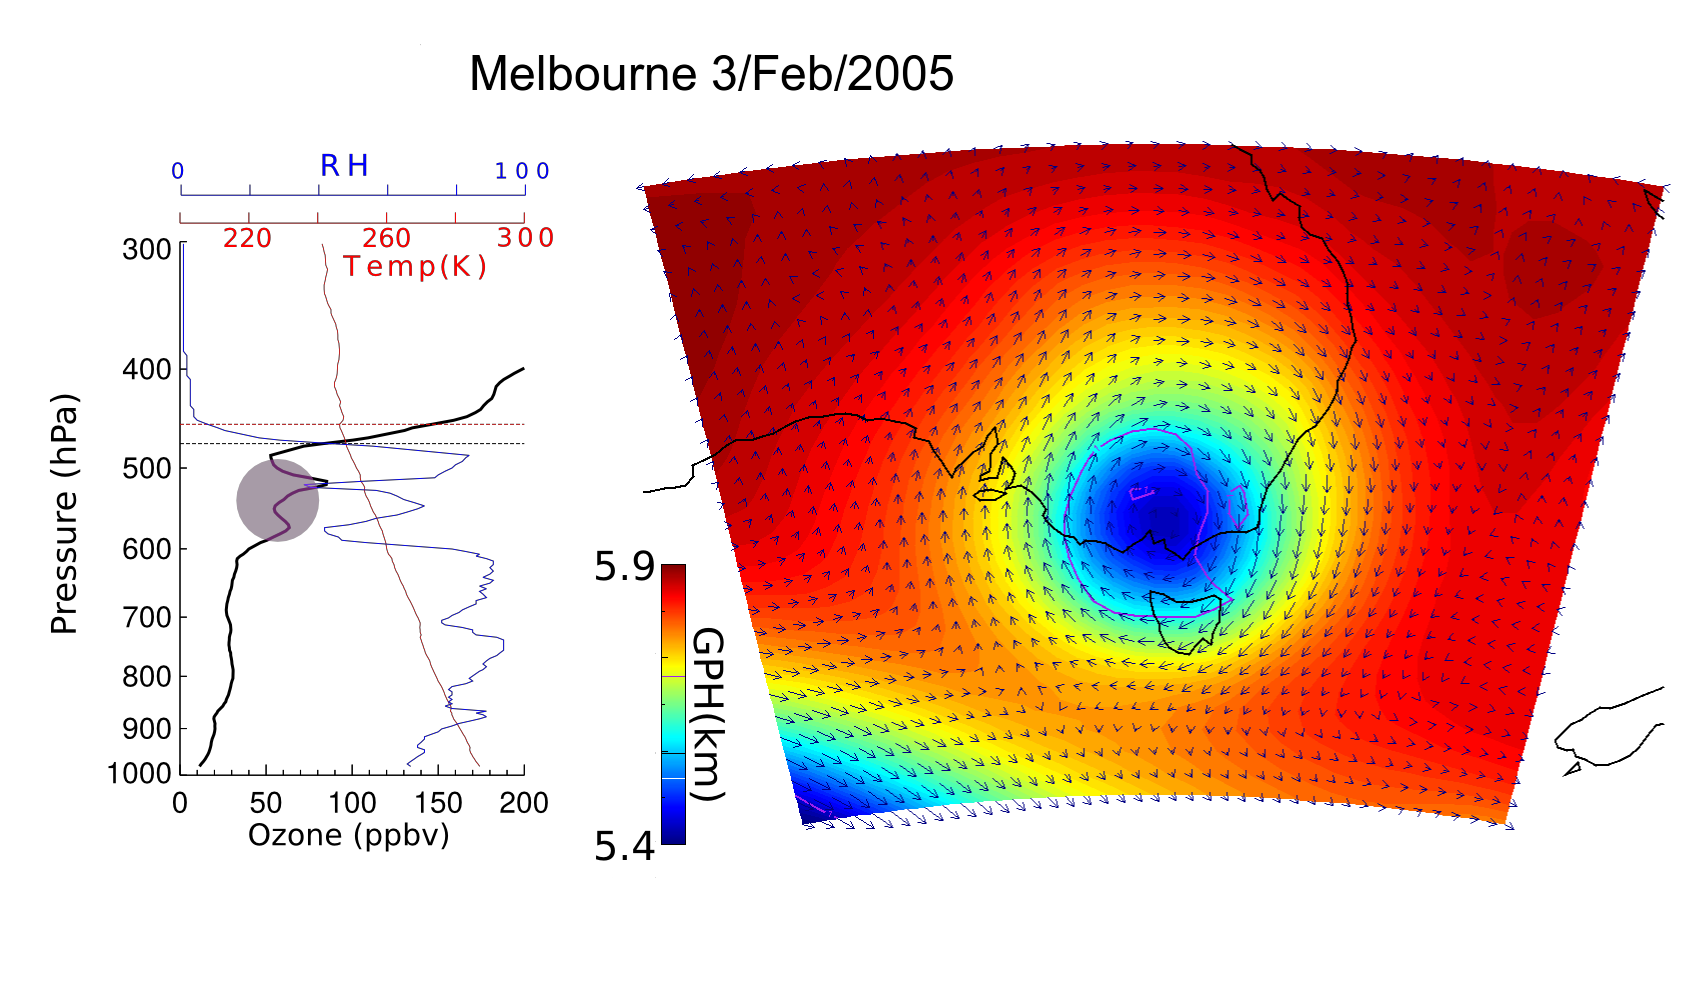
\includegraphics[width=1.0\columnwidth]{figures/Melbourne20050203.png}
      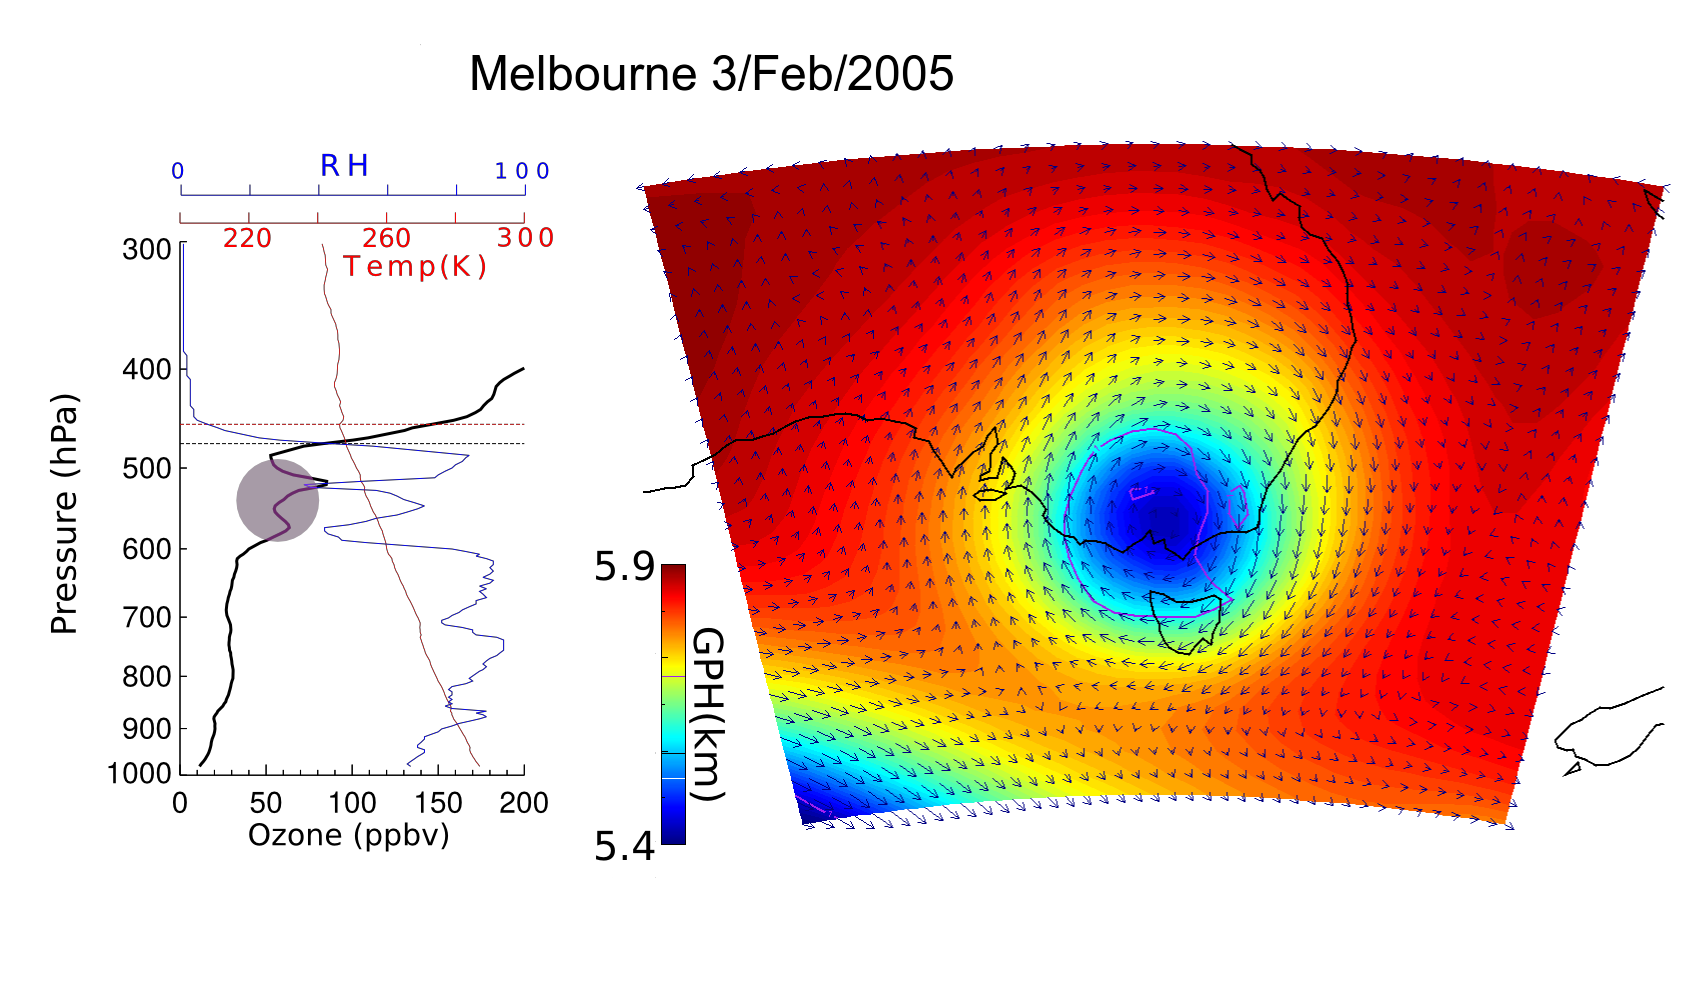
\includegraphics[width=12.0cm]{figures/Melbourne20050203.png}
      \caption{(Left) Vertical profile of ozone (black), relative humidity (blue), and temperature (red) measured by ozonesonde over Melbourne on 3 February 2005.
      The detected ozone STT event is highlighted in pink.
      Tropopause heights using both the ozone definition (black dashed line) and lapse rate definition (red dashed line) are also shown.
      (Right) Geopotential heights at 500 hPa from the ERA-Interim reanalysis, with wind vectors overplotted.
      Also shown are contours of potential vorticity units with 1 PVU in purple.}
      \label{fig:Melbourne20050203}
      
    \end{figure*}
    
    Figure \ref{fig:Melbourne20100113} (left) shows the ozone profile over Melbourne on 13 January 2010.
    The tropopause was higher on this date (120-160 hPa).
    Using our algorithm, we detected an ozone intrusion centred around 200~hPa.
    As before, ozone anti-correlation with relative humidity provides further evidence that the elevated ozone was stratospheric in origin.
    In this profile, there was clear separation between the detected intrusion (highlighted in pink) and the ozone tropopause (black dashed line), which indicates that the sonde passed through regular tropospheric air after hitting a stratospheric intrusion but before reaching the tropopause.
    The right panel shows that this event was associated with a trough (front) of low pressure  passing over southeastern Australia.
    This front traveled from west to east and caused a wave of lowered tropopause height. 
    Frontal passage is a known cause of STT as stratospheric air descends and streamers of ozone-rich air break off and mix into the troposphere \citep{Sprenger2003}.
    
    \begin{figure*}[t]
    % these IMAGE CREATED BY show_profile.py, EDITTED IN INKSCAPE
      
      %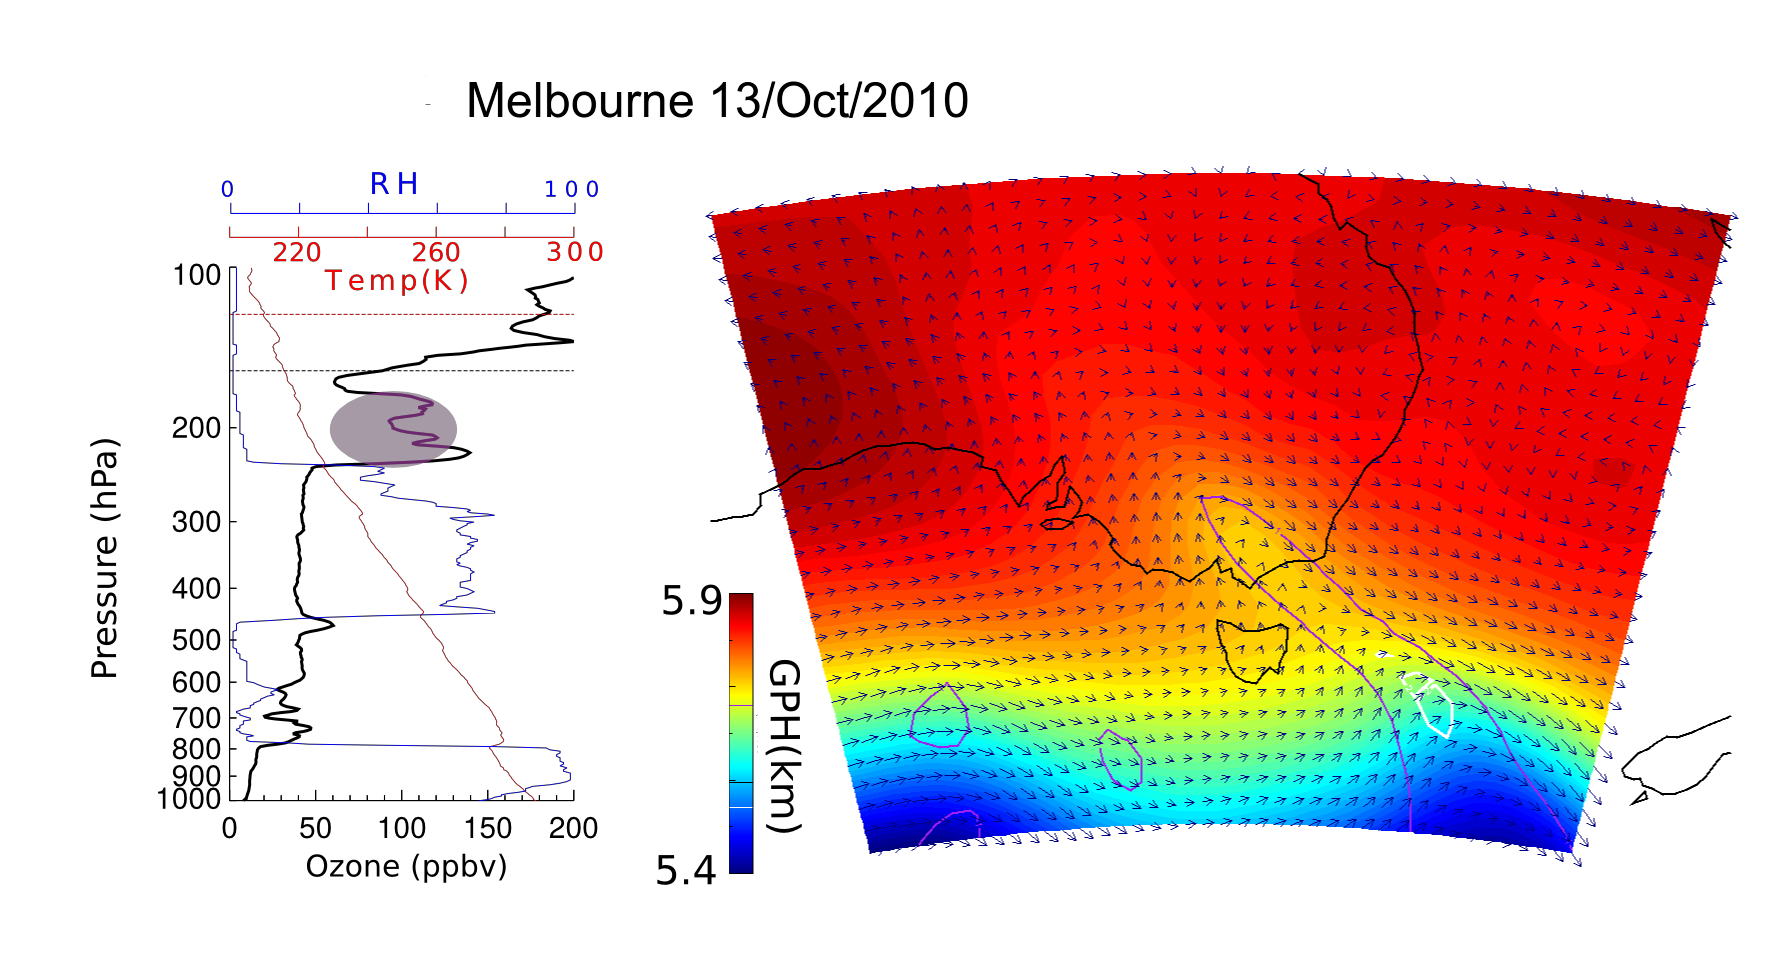
\includegraphics[width=1.0\columnwidth]{figures/Melbourne20100113.png}
      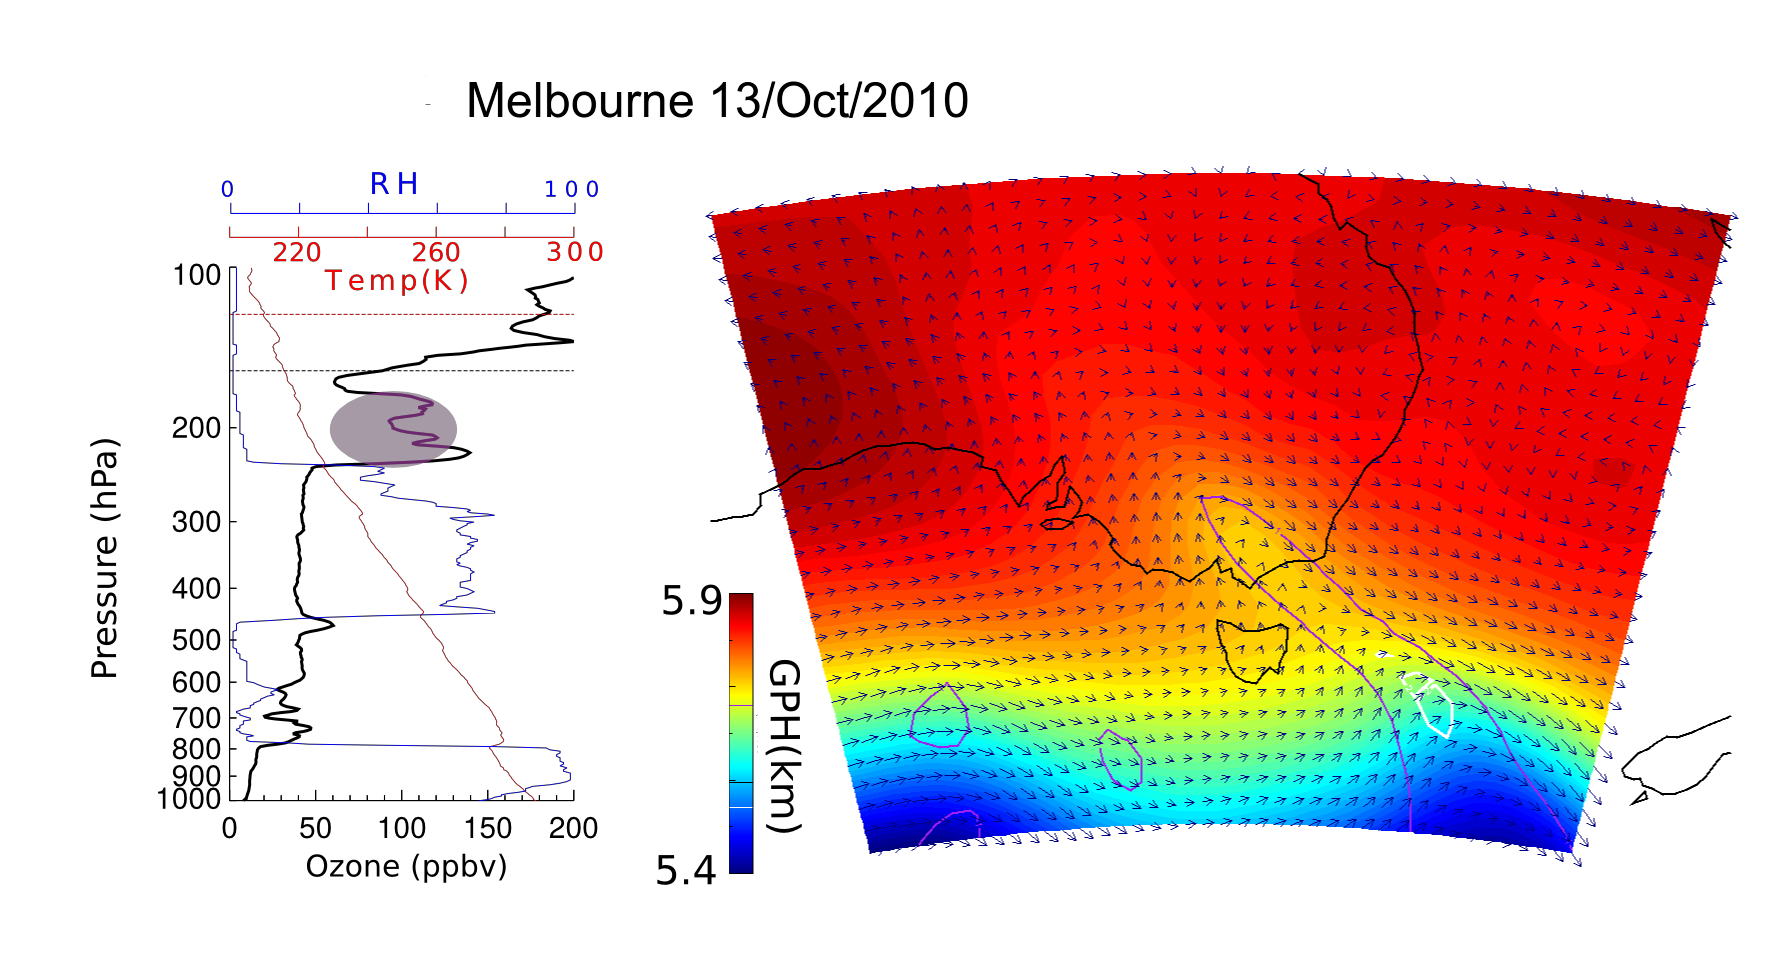
\includegraphics[width=12.0cm]{figures/Melbourne20100113.png}
      \caption{Same as Figure \ref{fig:Melbourne20050203} but for 13 January 2010.
	Also shown in this figure is the 2 PVU contour (white), often used to determine dynamical tropopause height.}
      \label{fig:Melbourne20100113}
      
    \end{figure*}

\section{STT event climatologies}
  \label{sec:eventclimatologies}
  Figure \ref{fig:SummarySeasonality} shows the seasonal cycles of STT frequency at Davis, Macquarie Island, and Melbourne.
  Frequency is determined as detected event count divided by total launched ozonesondes for each month.
  STT events in Figures \ref{fig:SummarySeasonality}-\ref{fig:SummaryTPDepths} are coloured based on the meteorological classification described in Sect. \ref{Section:WeatherClassifications}, with events classified as either low pressure fronts (“frontal”, dark blue), cut-off low pressure systems (“cutoff”, teal), or indeterminate (“misc”, cyan).
  Events that may have been influenced by transported smoke plumes (Sect. \ref{Section:BiomassBurning}) are shown in red.
  Ozonesonde releases are summarised in Table \ref{table:sondesummary} and detected event counts are summarised in Table \ref{table:EventCounts}.
  \begin{table}[t]
    %\centering
    \caption{Total number of ozonesonde detected STT events, along with the number of events in each category (see text).}
    \begin{tabular}{| c | c | c | c | c | c | c |} 
      \hline
      Site & Events & Cut-offs & Frontals & Misc & Fire \\
      \hline
      Davis     & 45 & 7  & 20 & 18 & 0 \\ 
      Macquarie & 47 & 10 & 20 & 9 & 8 \\
      Melbourne & 72 & 12 & 34 & 12 & 14 \\
      \hline
    \end{tabular}
    \label{table:EventCounts}
  \end{table}
  
  \begin{figure}[t]
  % these IMAGE CREATED BY non_transport_summary.py, labels edited IN INKSCAPE
    
    %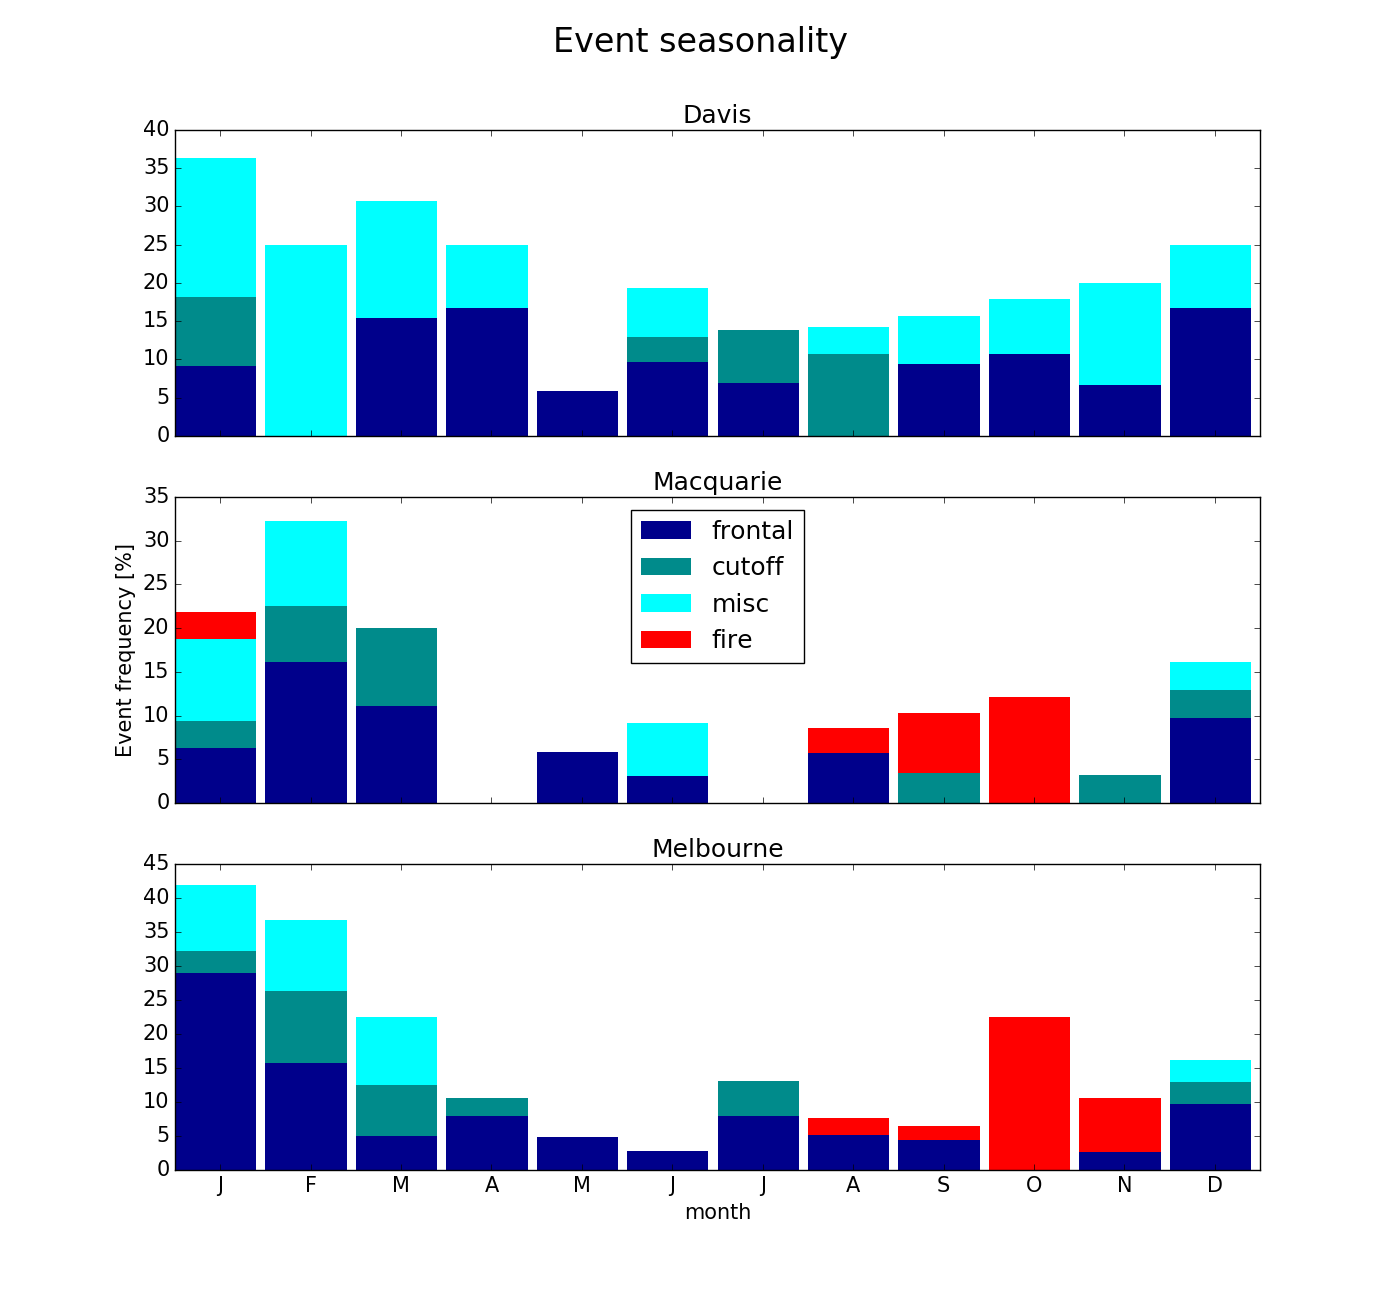
\includegraphics[width=1.0\columnwidth]{figures/summary_season.png}
    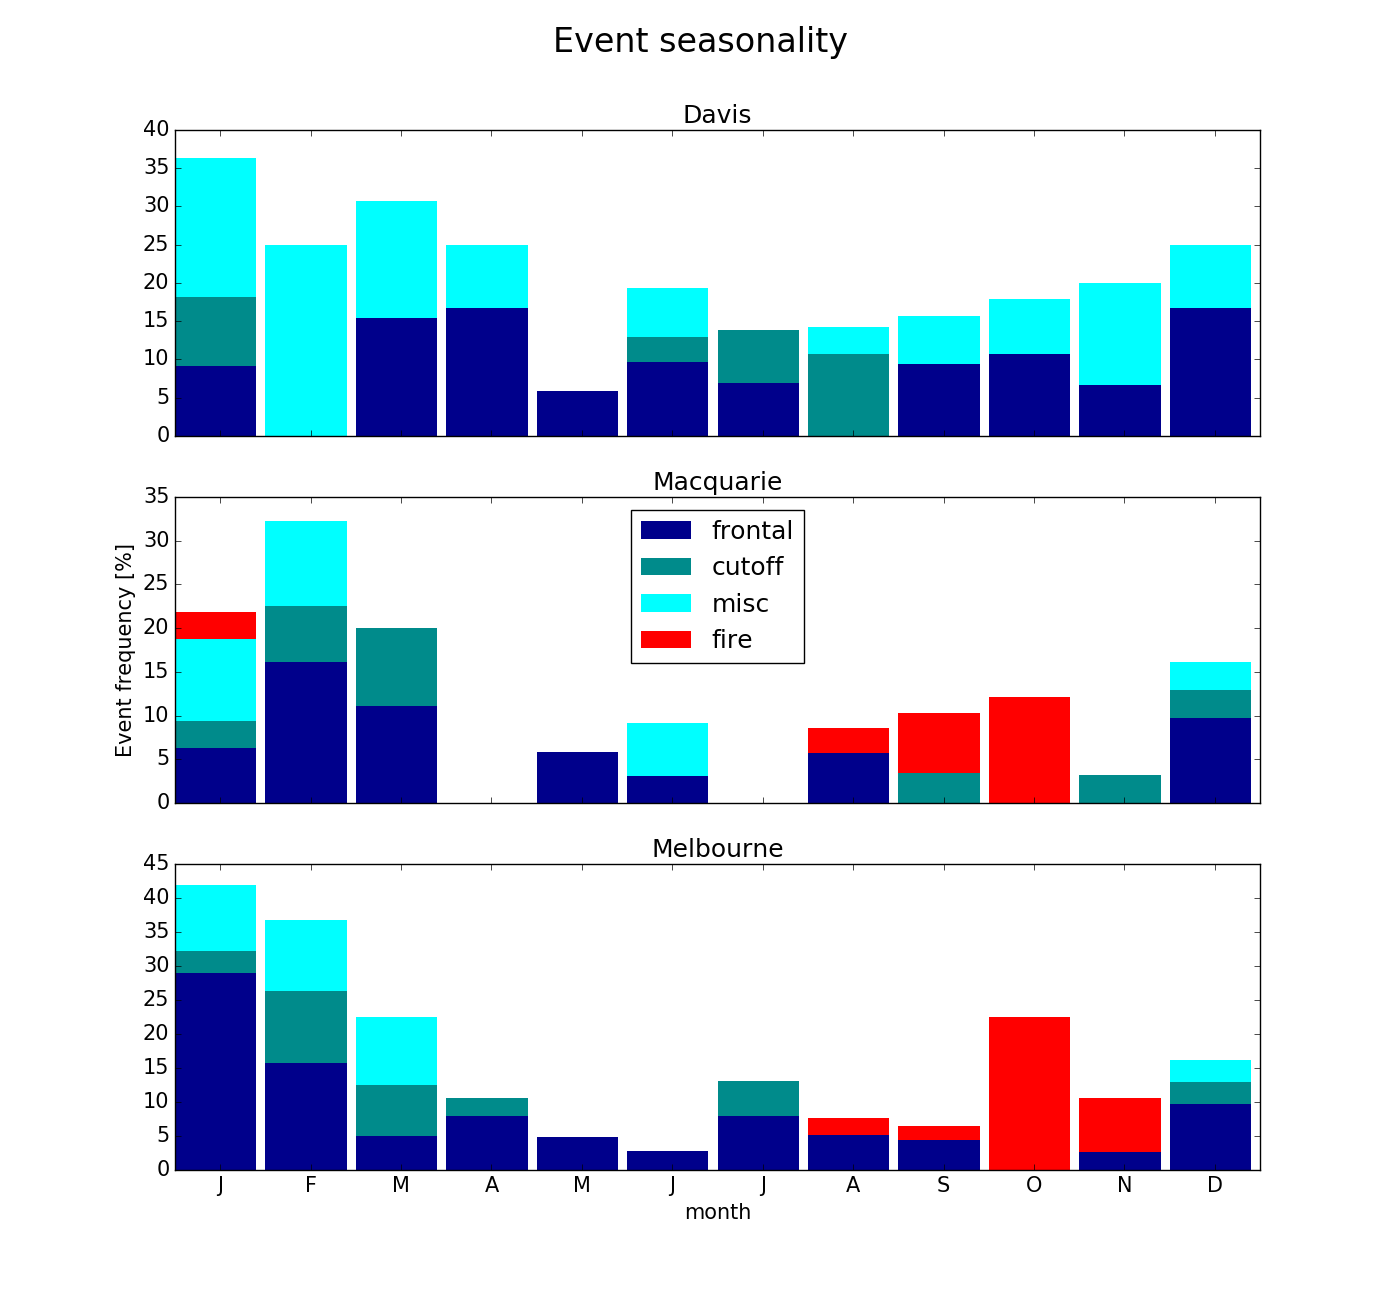
\includegraphics[width=8.3cm]{figures/summary_season.png}
    \caption{Seasonal cycle of STT event frequency at Davis (top), Macquarie Island (middle), and Melbourne (bottom).
      Events are categorised by associated meteorological conditions as described in the text, with low pressure fronts (“frontal”) in dark blue, cut-off low pressure systems (“cutoff”) in teal, and indeterminate meteorology (“misc”) in cyan. 
      Events that may have been influenced by transported smoke plumes are shown in red (see text for details).}
    \label{fig:SummarySeasonality}
    
  \end{figure}
  
  There is an annual cycle in the frequency of STT events  (Fig. \ref{fig:SummarySeasonality}) with a summertime peak above all three sites.
  This summertime peak is due to a prevalence of summer low-pressure storms and fronts, which increase turbulence and lower the tropopause \citep{Reutter2015}.
  For all three sites, STT events mainly occur in summer, and are most commonly associated with low pressure synoptic systems.
  At Davis, there is increased Antarctic winter activity, which may be due to the polar vortex and its' associated lowered tropopause and increased turbulence.
  STT events associated with cut-off low pressure systems are more prevalent during summer (winter for Davis), while STT events associated with frontal passage occur throughout the year.

  %The increased winter time frequency of STT events at Davis (relative to Macquarie and Melbourne) may be due to increased polar jet stream activity at this time.
  
  To examine the robustness of the distributions shown in Fig \ref{fig:SummarySeasonality}, we developed an alternative assessment of the seasonal occurrence of STT events, with results shown in Figure \ref{fig:AndrewProxySTT}.
  Here STT occurrence is evaluated by consideration of the square of the dry Brunt-Viäsälä frequency (N$^2$) at the heights of the ozone tropopause (z$_{OT}$) and lapse rate tropopause (z$_{LRT}$) in each ozonesonde profile that has been binned to 500~m resolution.
  We use N$^2$ to assess atmospheric stability, which is normally distinctly higher in the stratosphere than in the troposphere, and assume that the vertical temperature gradients within the intrusion respond most rapidly to transported heat, which is an additional characteristic of stratospheric air.
  The altitude binning chosen is a compromise between vertical resolution and the level of variability in N$^2$ introduced by temperature gradients associated with perturbations from gravity waves and changes near the lapse rate tropopause, and is the minimum that produces a robust seasonal distribution.
  We define STT as having taken place if N$^2$(z$_{OT}$) $>$ N$^2$(z$_{LRT}$) and z$_{OT}$ $<$ z$_{LRT}$; in this way the characteristically higher static stability and ozone concentration of stratospheric intrusion is regarded as being retained as it penetrates below the lapse rate tropopause. 
  The seasonal distributions shown for the three stations in Fig. \ref{fig:AndrewProxySTT} are generally similar to those shown in Fig. \ref{fig:SummarySeasonality} (although detected events are less frequent), with the main exception that no events are identified with the alternative method at Davis in the first half of the year.
  From December to June, ozonesondes are generally only launched monthly at Davis, and the lack of STT events in these months for Davis potentially reflects the fewer measurement opportunities.
  
  \begin{figure}[t]
    % Figure from Andrew Klekociuk excel barplot
    
    %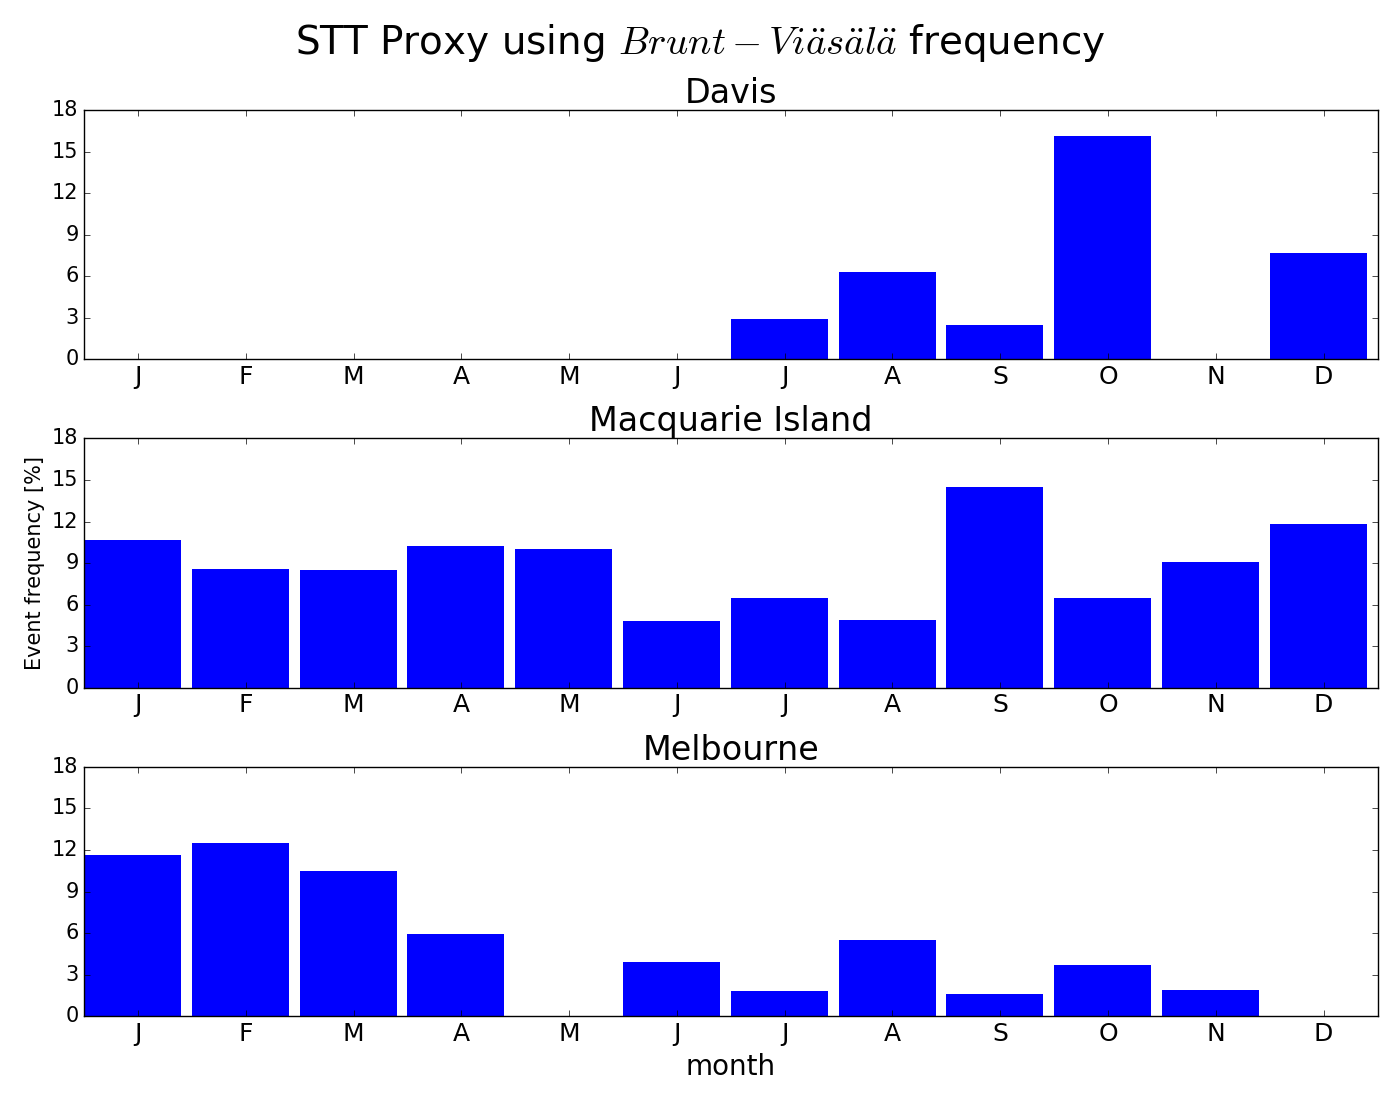
\includegraphics[width=0.8\columnwidth]{figures/AndrewProxySTT.png}
    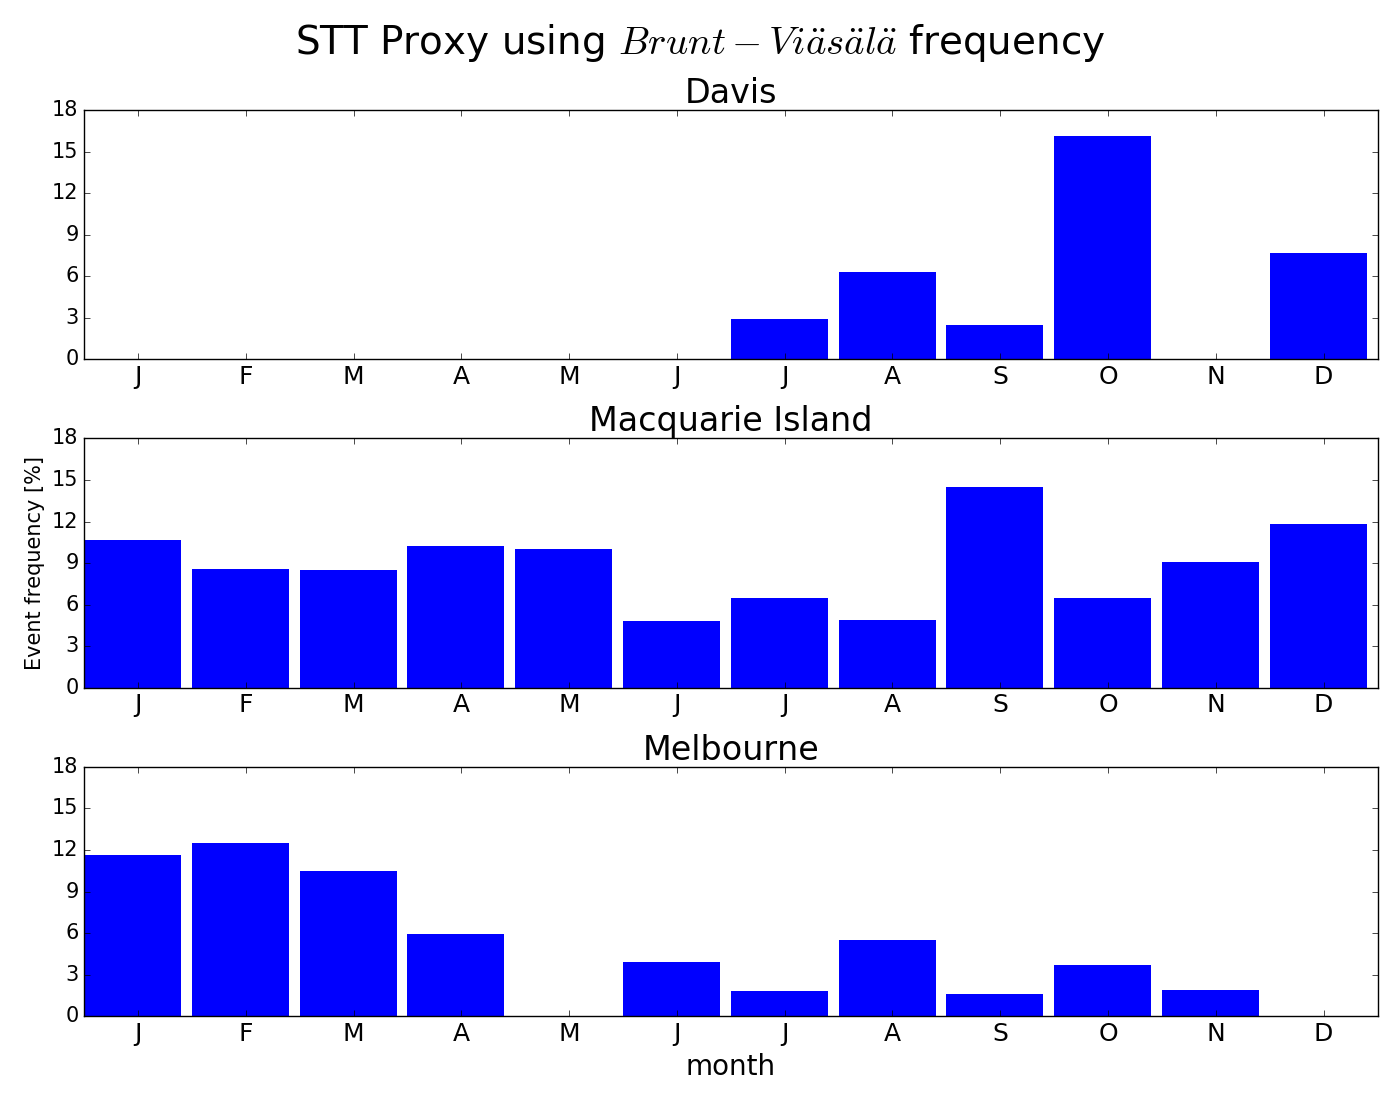
\includegraphics[width=8.3cm]{figures/AndrewProxySTT.png}
    \caption{Seasonal distribution of the alternative STT proxy, obtained from consideration of the static stability at the ozone and lapse rate tropopauses, for Davis (2003-2012), Macquarie Island (1994-2012) and Melbourne (1999-2012).}
    \label{fig:AndrewProxySTT}
    
  \end{figure}
  
  Figure \ref{fig:SummaryAltitudes} shows the altitudes of detected events, based on the altitude of peak (local maximum ozone within enhancement altitude) tropospheric ozone in the ozonesonde profile.
  STT event peaks most commonly occur at 6--10~km above Melbourne and 6--9~km at Davis but are distributed more evenly at Macquarie Island from ~4--7.5 km.
  There is no clear relationship between meteorological conditions and event altitude.
  
  \begin{figure}[t]
    %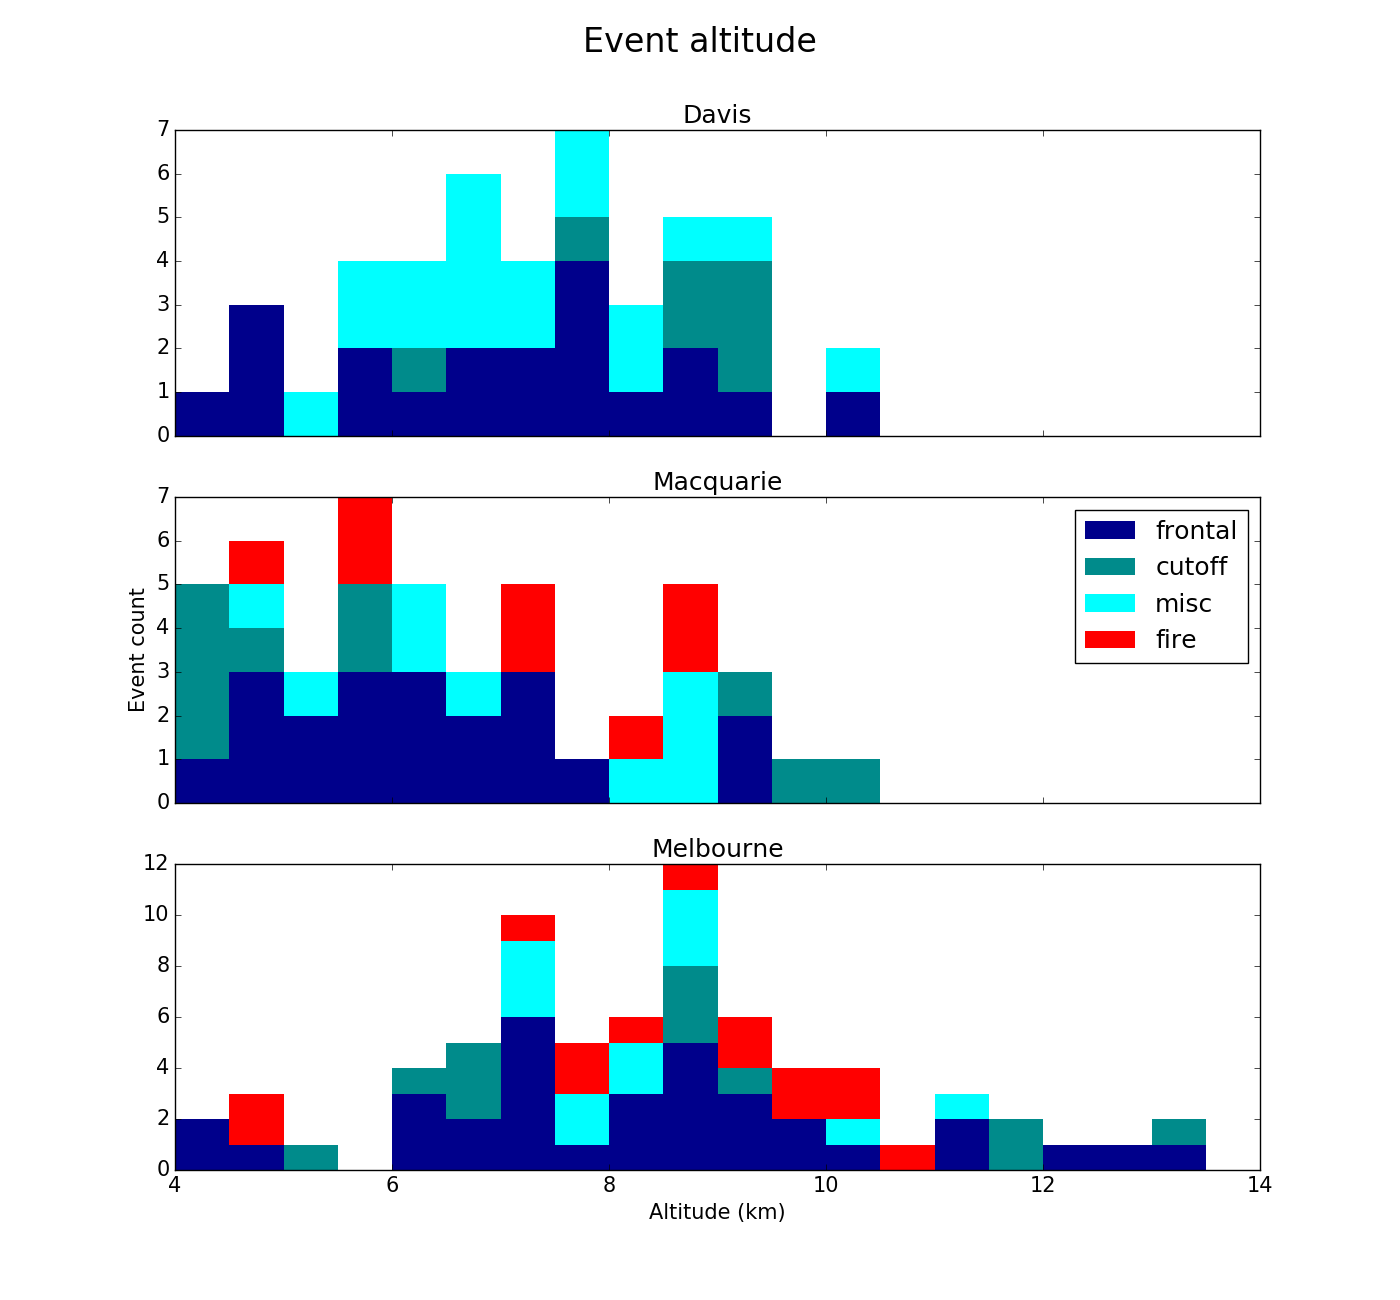
\includegraphics[width=0.99\columnwidth]{figures/summary_altitude.png}
    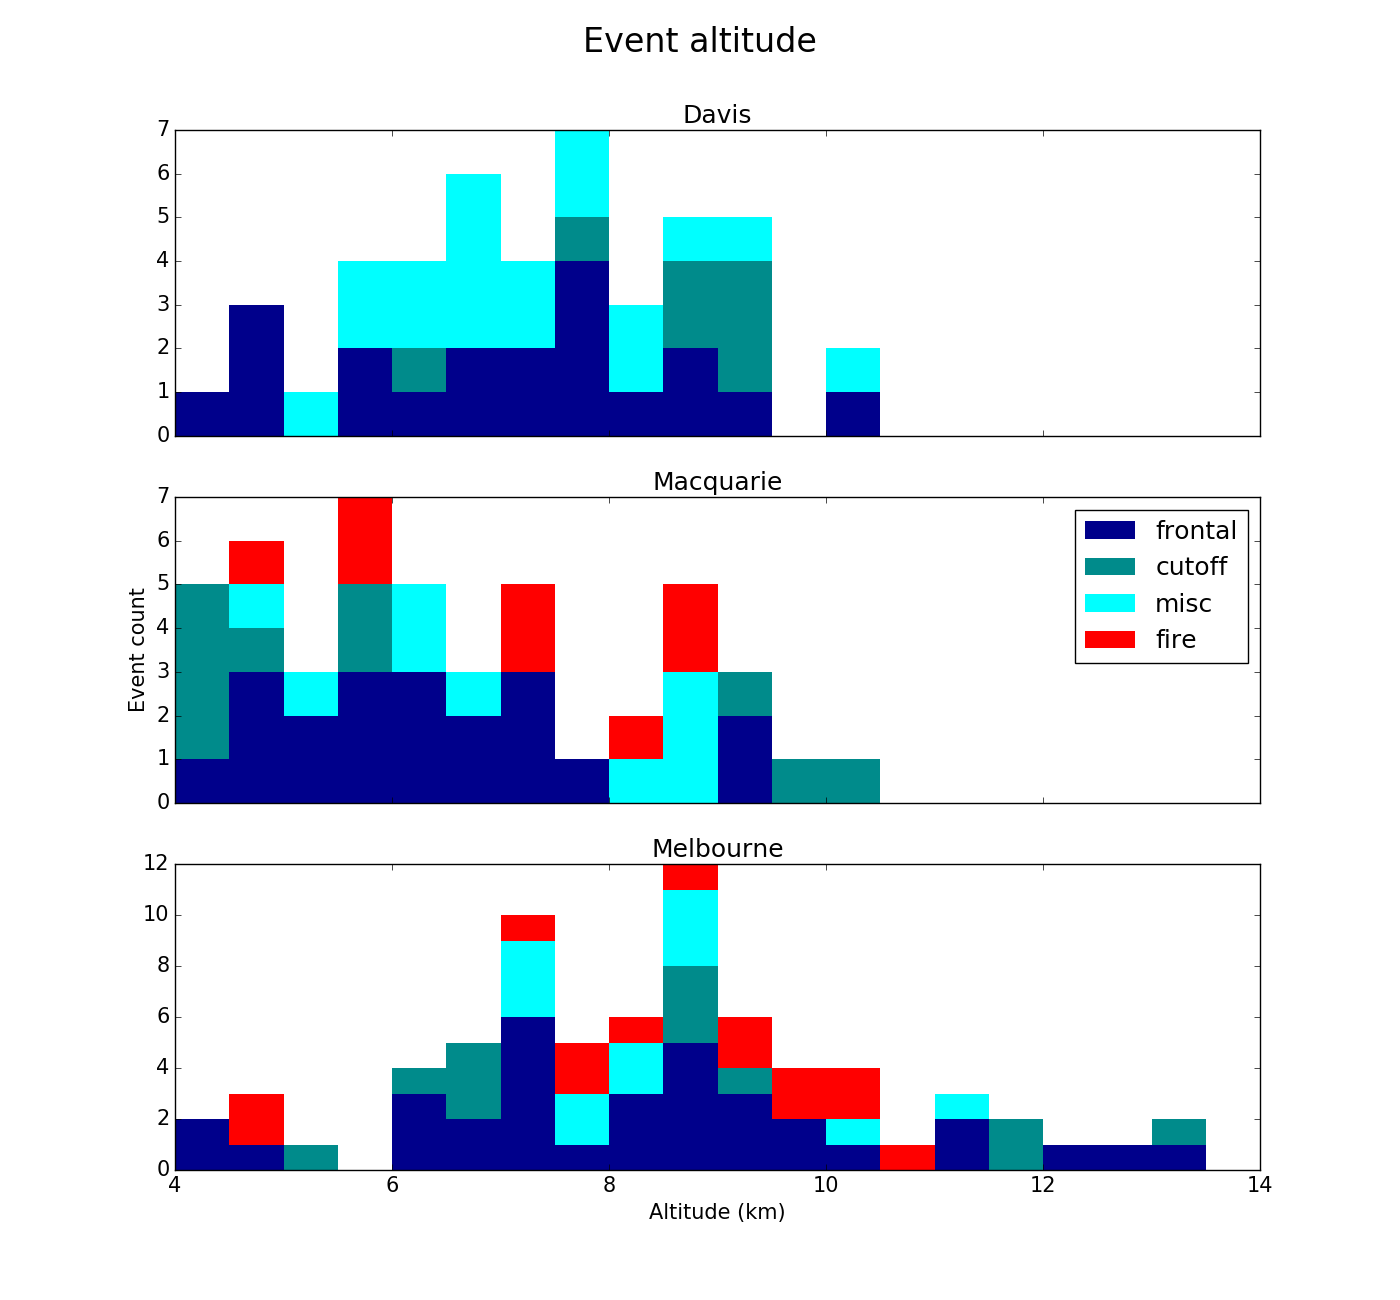
\includegraphics[width=8.3cm]{figures/summary_altitude.png}
    \caption{The distribution of STT event altitude at Davis (top), Macquarie Island (middle), and Melbourne (bottom), determined as described in the text.
    Events are coloured as described in Fig. \ref{fig:SummarySeasonality}.}
    \label{fig:SummaryAltitudes}
  \end{figure}

  Figure \ref{fig:SummaryTPDepths} shows the distance from the tropopause of the event peak (using the lowest of the two tropopause definitions).
  The majority of STT events occur within 3~km of the tropopause at Macquarie Island, and within 2~km of the tropopause at Davis. 
  Over Melbourne, the event depth is more spread out, and peak ozone enhancement generally occurs within 6~km of the tropopause.
  Again, there is no clear relationships between meteorological conditions and event depth.

  \begin{figure}[t]
    
    %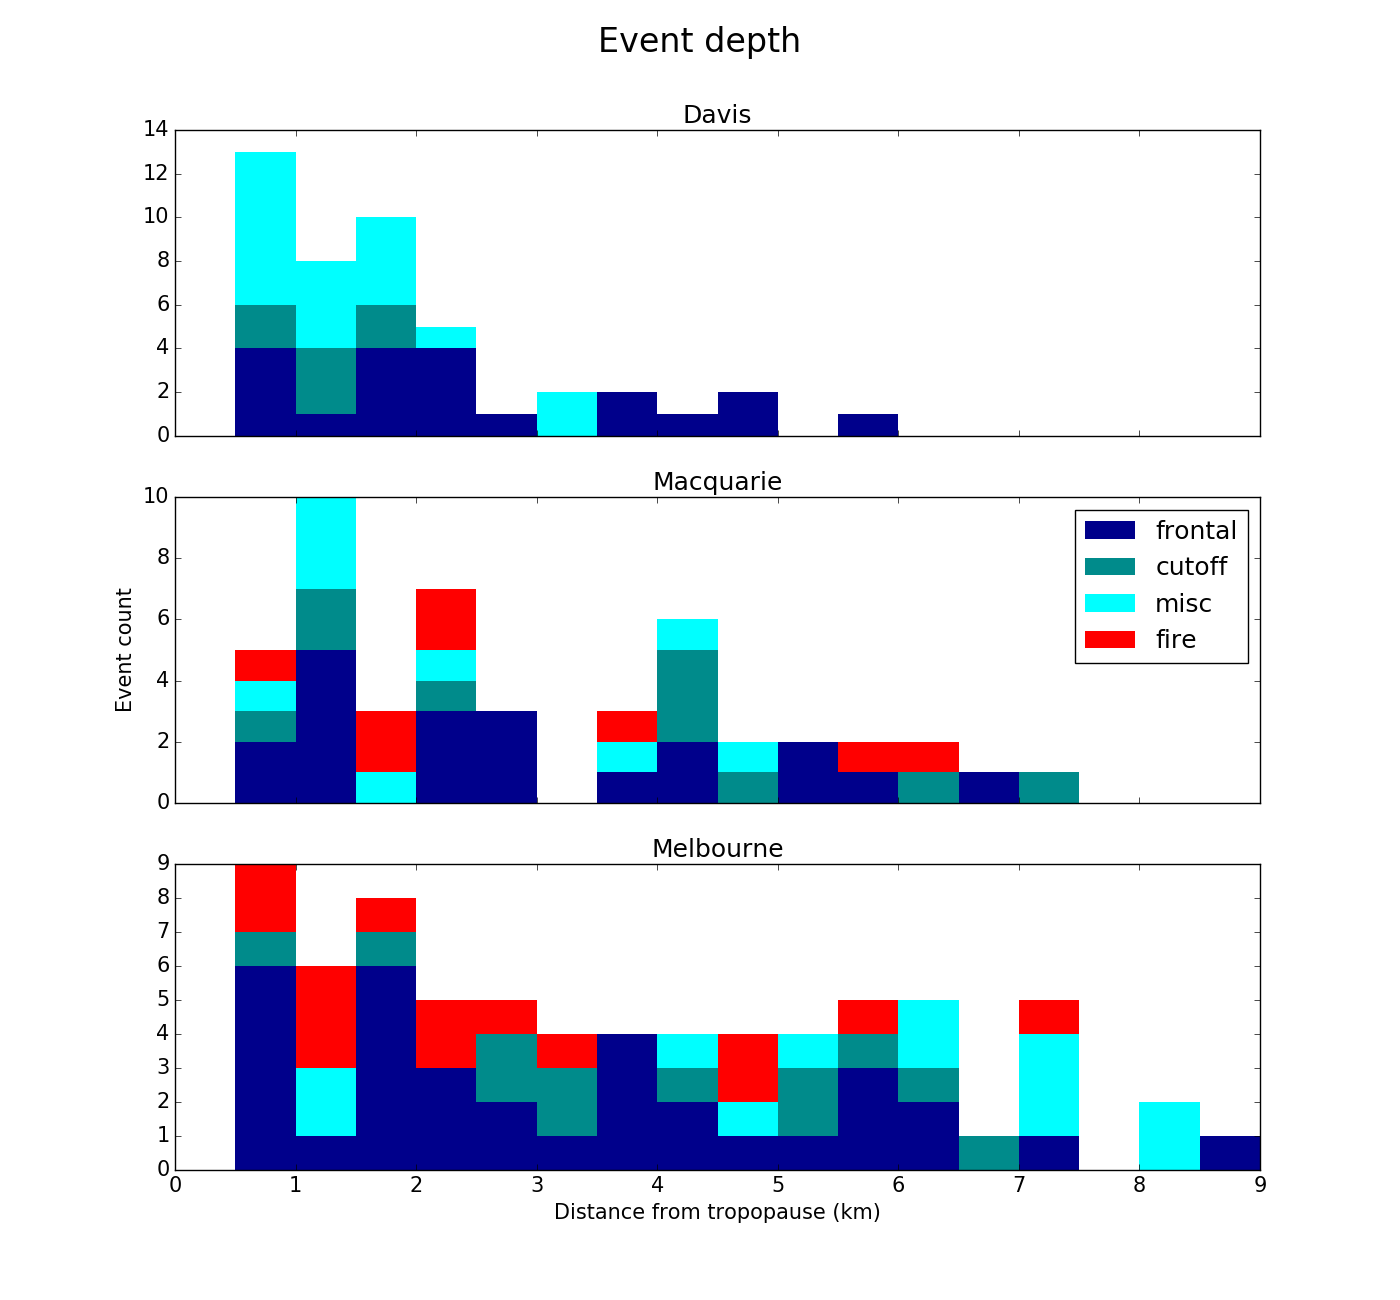
\includegraphics[width=0.99\columnwidth]{figures/summary_depth.png}
    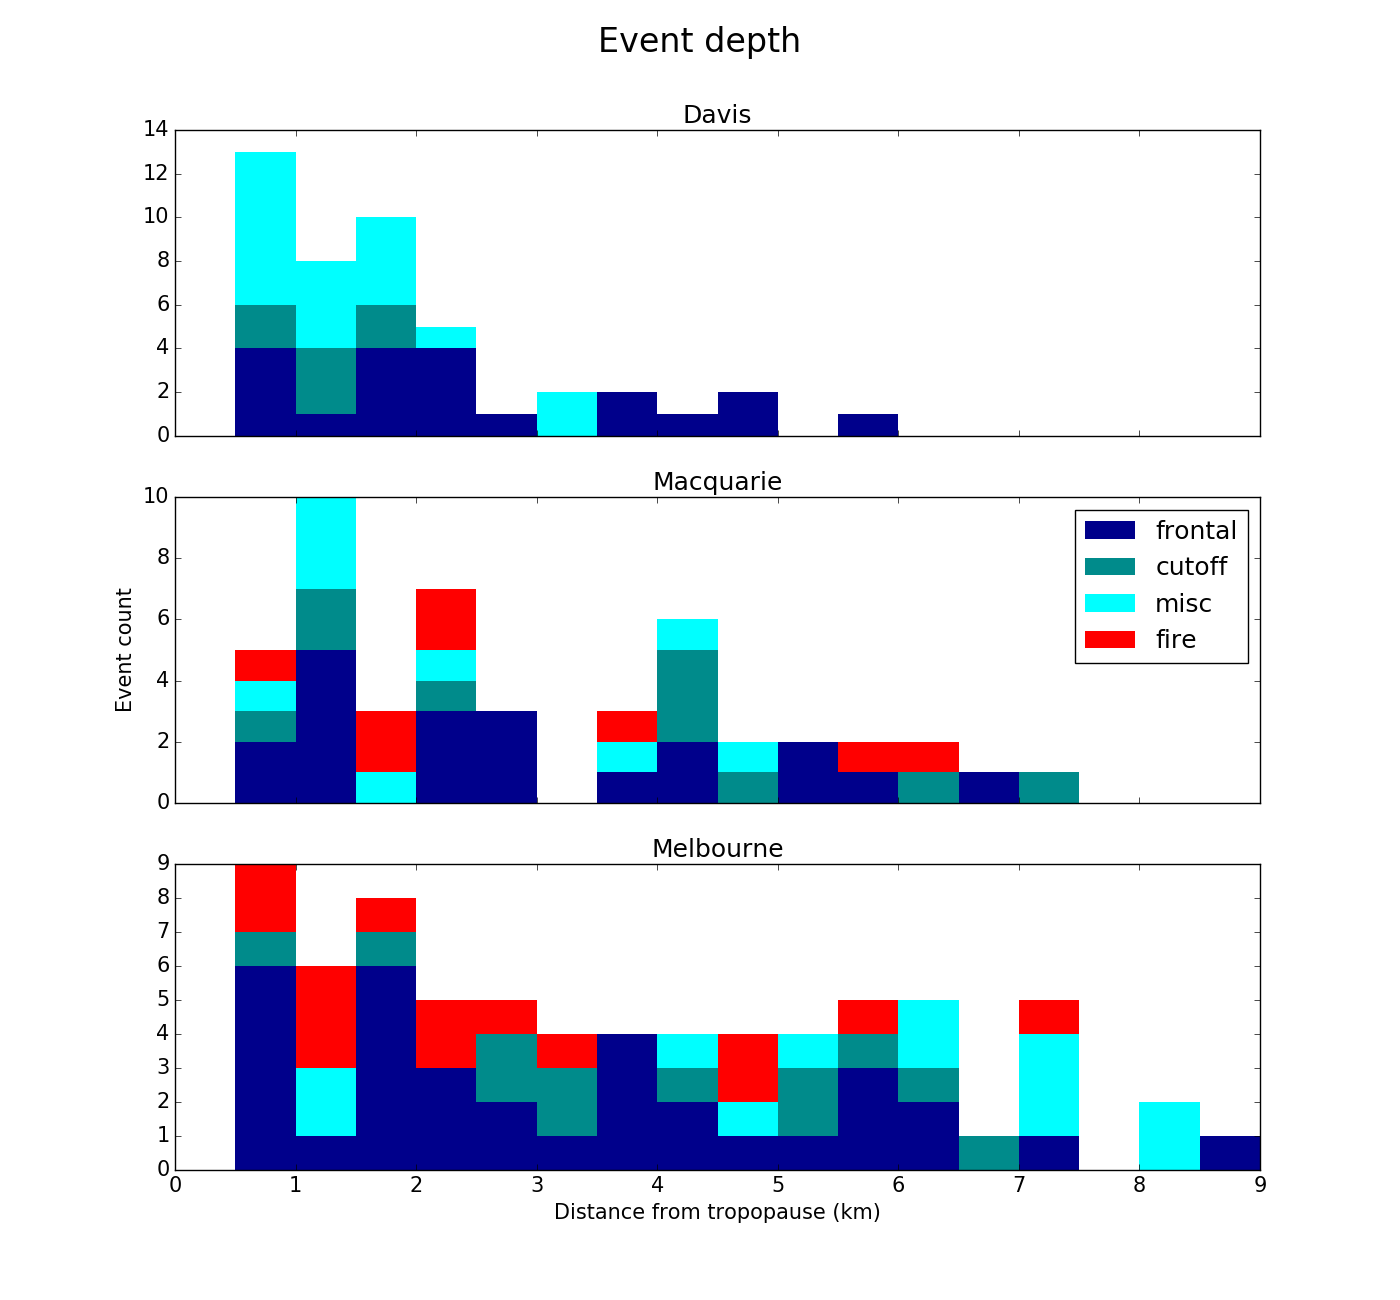
\includegraphics[width=8.3cm]{figures/summary_depth.png}
    \caption{The distribution of STT event distance from the tropopause at Davis (top), Macquarie Island (middle), and Melbourne (bottom), determined as described in the text.
    Events are coloured as described in Fig. \ref{fig:SummarySeasonality}.}
    \label{fig:SummaryTPDepths}
    
  \end{figure}

\section{Simulation of southern mid-latitude ozone columns}
  
  Figure \ref{fig:StationSeriesGEOSChem} compares the time series of tropospheric ozone columns ($\Omega_{O_3}$) in molecules cm$^{-2}$ simulated by GEOS-Chem (red) to the measured tropospheric ozone columns (black).
  Observed tropospheric columns are calculated from the ozonesondes by calculating the ozone number density (molec cm$^{-3}$) using measured ozone partial pressure (P$_{O_3}$) and integrating over the measured GPH up to the tropopause:
  \begin{equation*}
    %\frac{n_{O_3}}{V} &=& \frac{P_{O_3}}{RT} \\
    %\mathbf{\Omega_{O_3}} = \int_{0}^{\text{TP}} \frac{n_{O_3}}{V} \times N_{Av} \text{d}z
    \mathbf{\Omega_{O_3}} = \int_{0}^{\mathrm{TP}} \frac{P_{O_3}(z)}{R \times T(z)} \times N_{Av} \mathrm{d}z
  \end{equation*}
  Where z is the altitude (GPH), TP is the altitude at the tropopause, T is the temperature, R is the ideal gas constant, and N$_{Av}$ is Avegadros constant.
  In both observations and model, the maximum ozone column at Melbourne occurs in austral summer, with a minimum in winter, while Macquarie and Davis show the opposite seasonality.
  
  \begin{figure*}[t]
    % made in examine_stations.py in stations repository
    %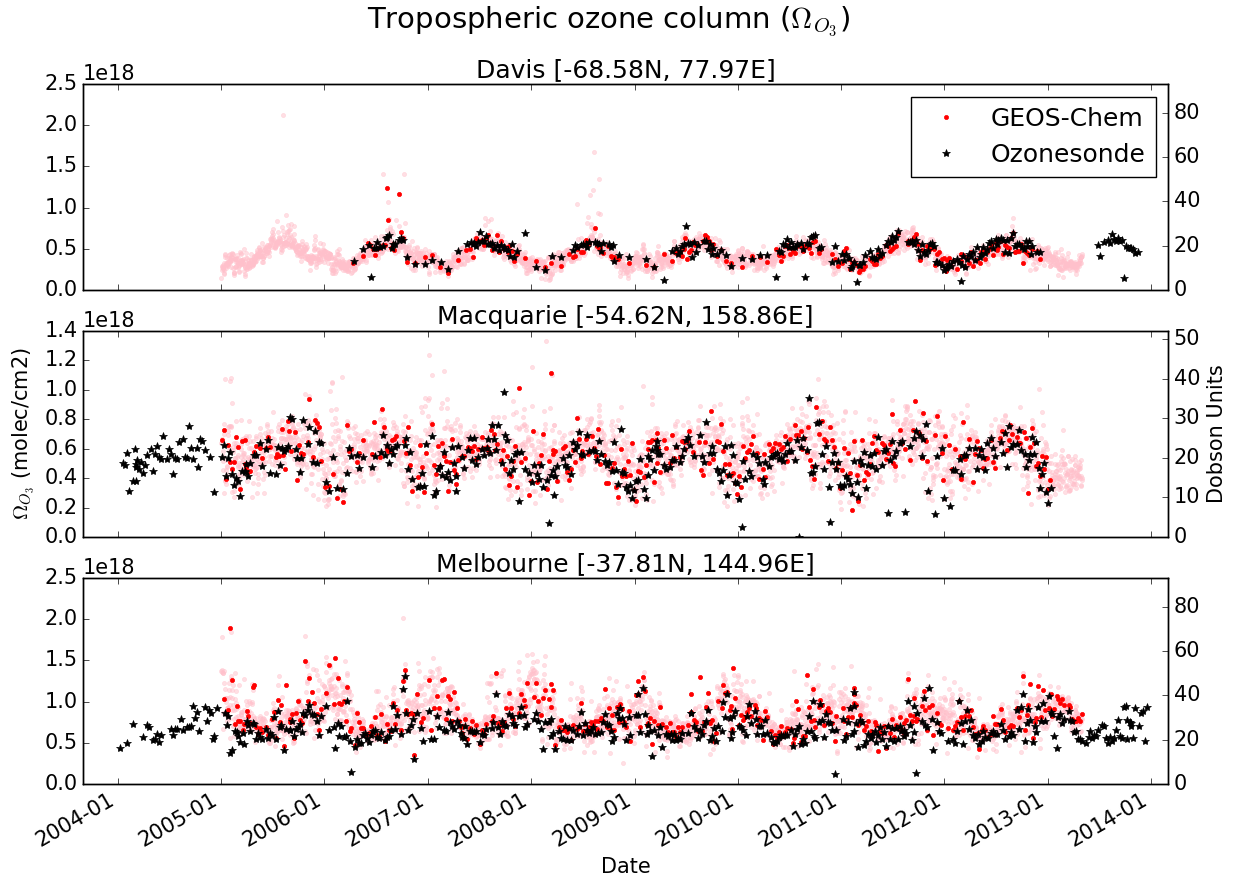
\includegraphics[width=\textwidth]{figures/StationSeries.png}
    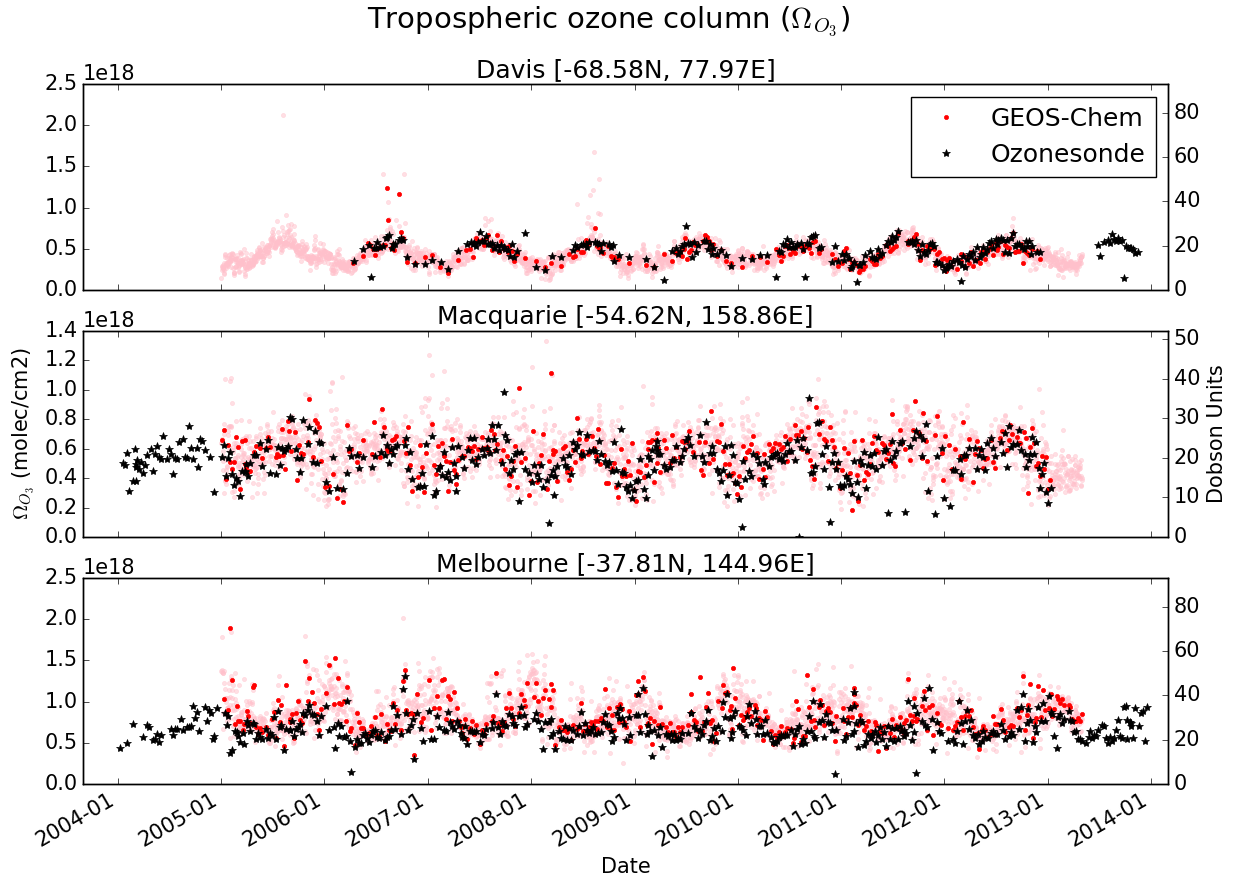
\includegraphics[width=12.0cm]{figures/StationSeries.png}
    \caption{Comparison between observed (black) and simulated (pink, red) tropospheric ozone columns ($\Omega_{O3}$, in molecules cm$^{-2}$) from 1 January 2004 to 30 April 2013.
    For the model, daily output is shown in pink, while output from days with ozonesonde measurements are shown in red.
    For each site, the model has been sampled in the relevant grid square.}
    %Columns calculated from ozonesondes are shown as black stars, each representing one measurement.}
    \label{fig:StationSeriesGEOSChem}
  \end{figure*}
  
  GEOS-Chem provides a reasonable simulation of the observed seasonality and magnitude of $\Omega_{O_3}$. 
  Reduced major axis regression of observed versus simulated $\Omega_{O_3}$ gives a line of best fit with slopes being 1.08 for Davis, 0.99 for Macquarie, and 1.34 for Melbourne.
  The model is only partially able to reproduce the variability in the observations, with paired r$^2$ values for of 0.38 for Davis, 0.18 for Macquarie, and 0.37 for Melbourne.
  Much of the variability is driven by the seasonal cycle, and after removing this effect (by subtracting the multi-year monthly means), the r$^2$ values decrease to .07, .11, .30 respectively, although the slope improves at Melbourne to 1.08.
  %The model shows more day-to-day variability than the ozonesondes (MAYBEDO: Verify this), although there are daily simulated values for the model while only weekly or less for the ozonesondes.
  
  \begin{figure*}[t]
    % Created in examine_stations.py
    %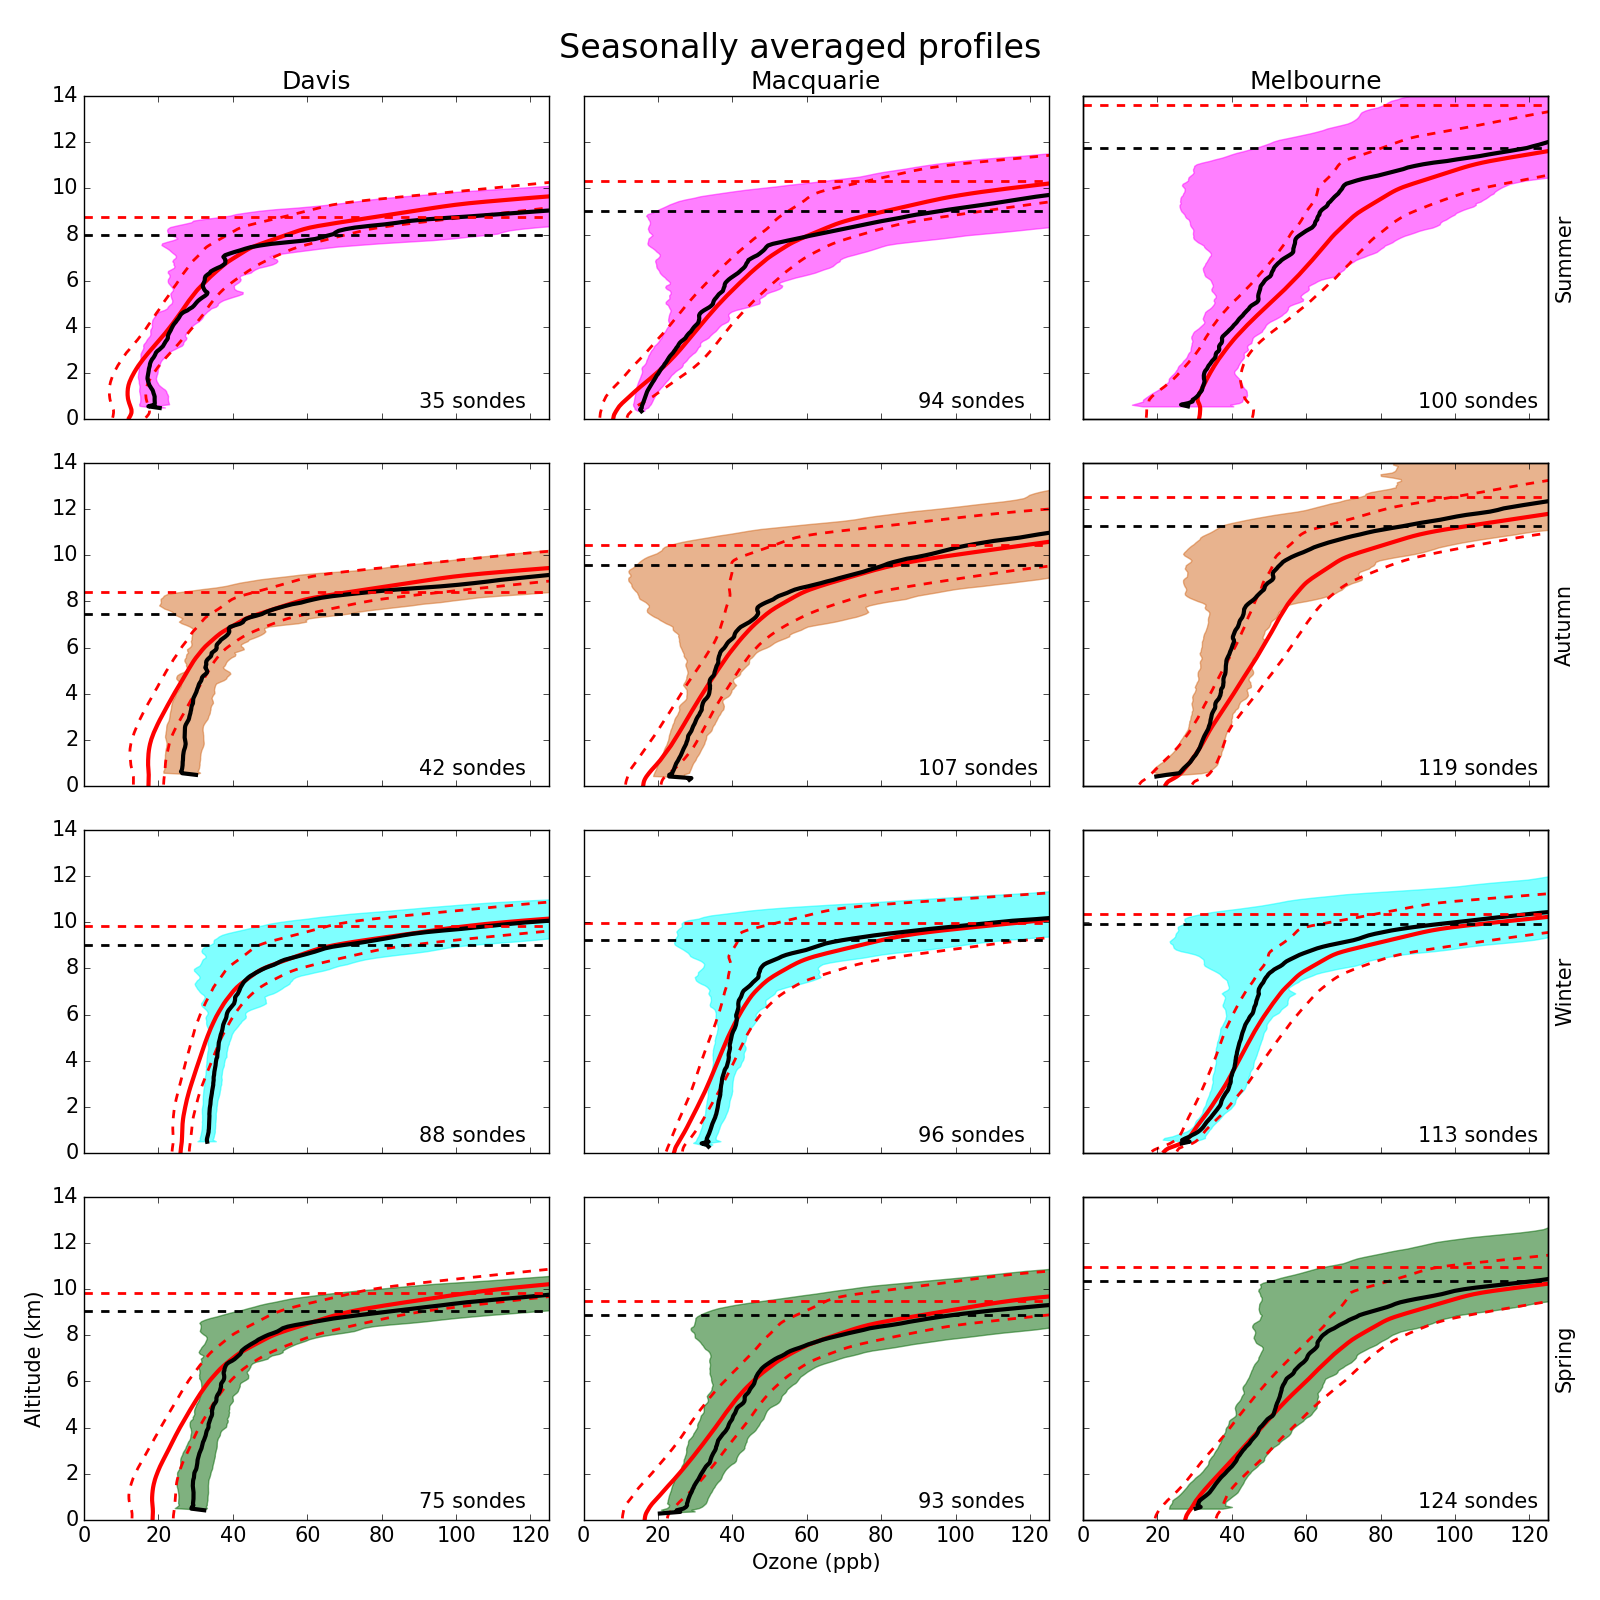
\includegraphics[width=\textwidth]{figures/seasonalprofiles00.png}
    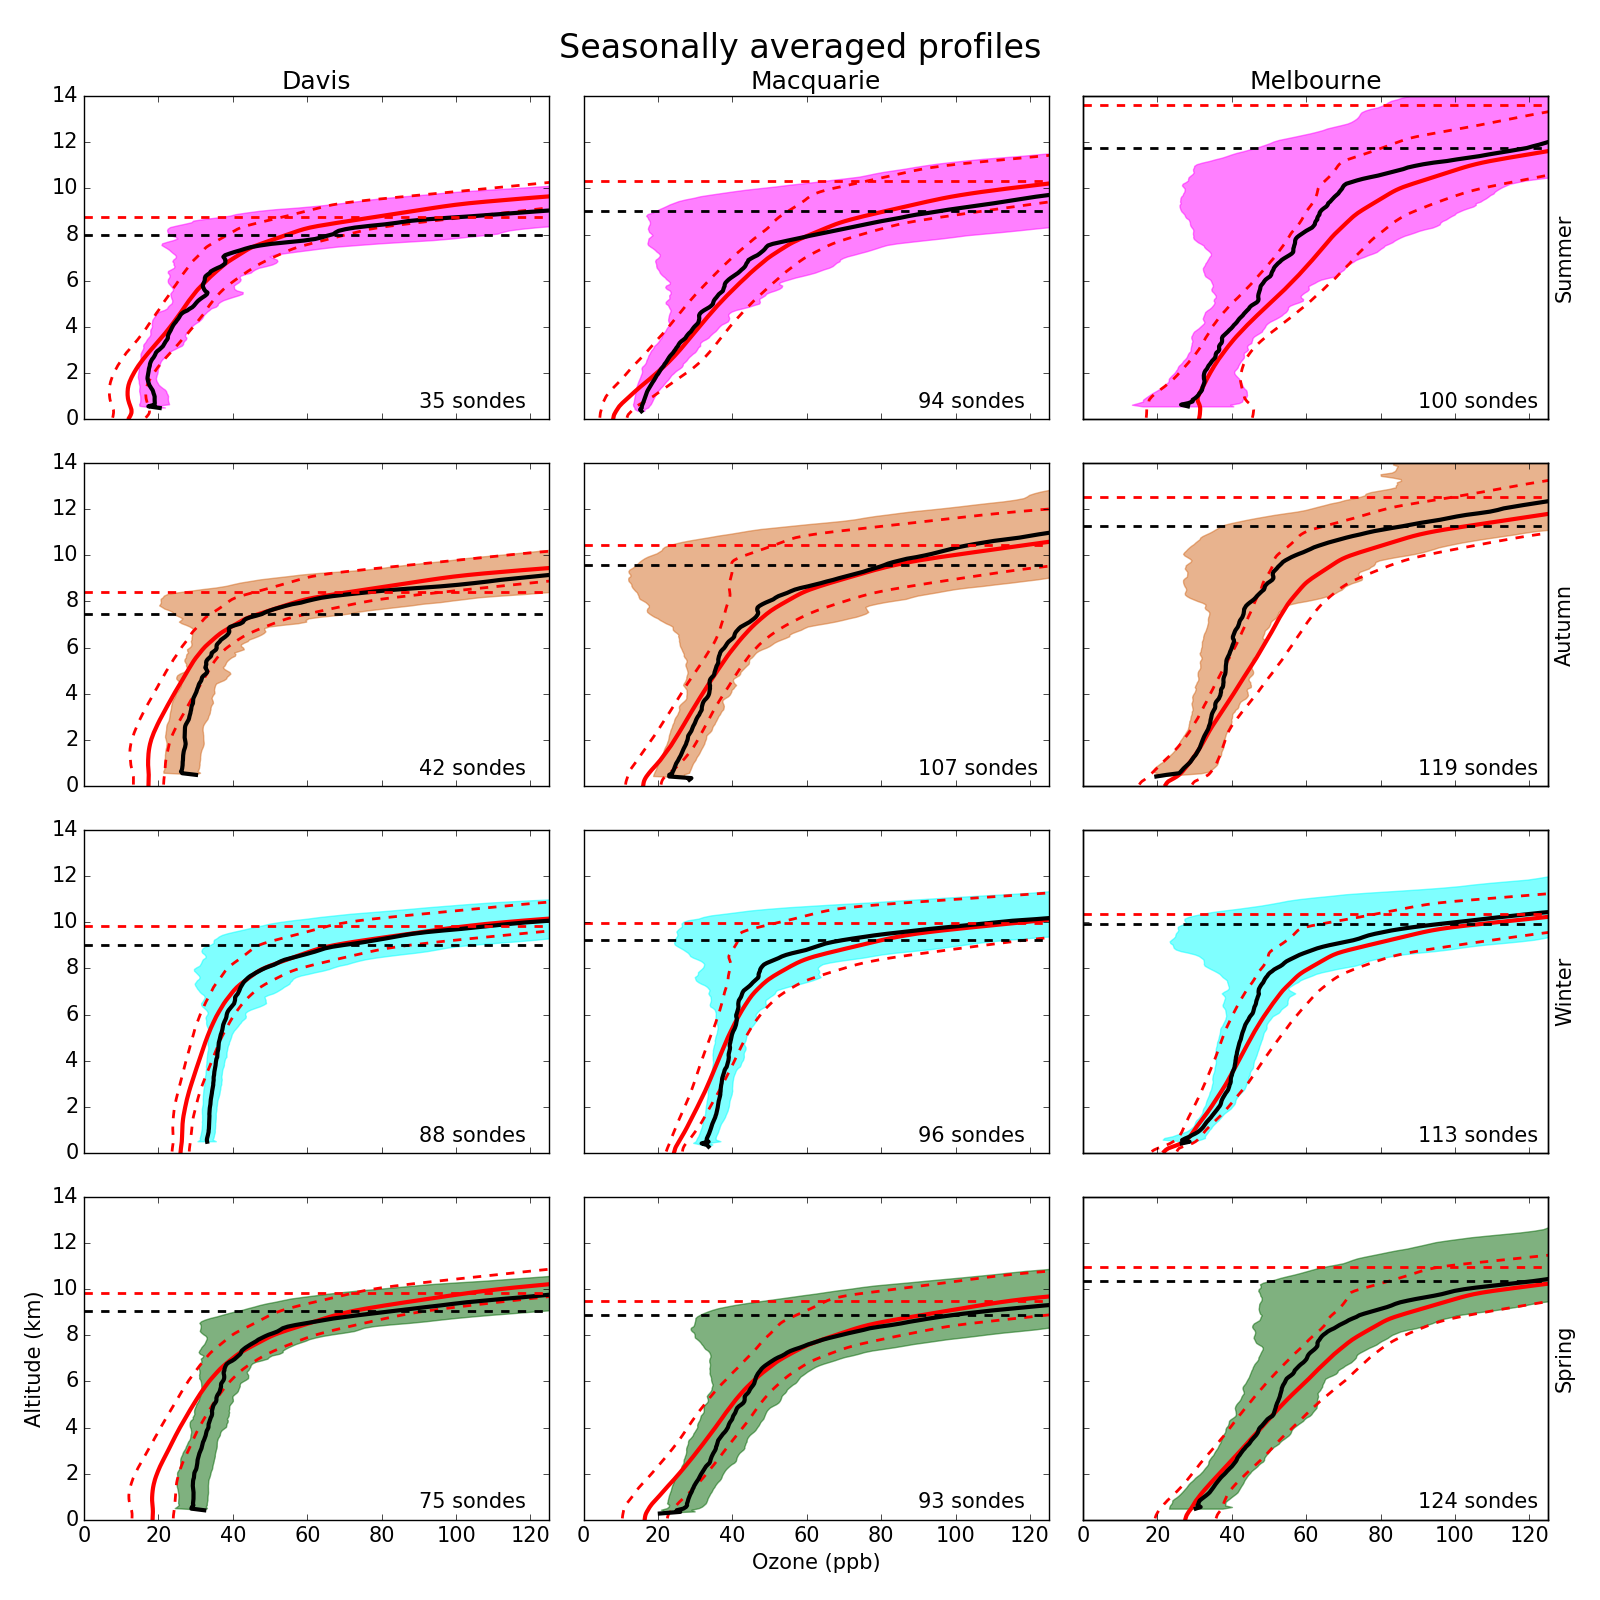
\includegraphics[width=12.0cm]{figures/seasonalprofiles00.png}
    \caption{Observed and simulated tropospheric ozone profiles over Davis, Macquarie, and Melbourne, averaged seasonally.
    Model means (2005-2013 average) are shown as red solid lines, with red dashed lines showing the 10th and 90th percentiles.
    Ozonesonde means (over each season, for all years) are shown as black solid lines, with coloured shaded areas showing the 10th and 90th percentiles.
    The horizontal dashed lines show the mean tropopause heights from the model (red) and the observations (black).}
    \label{fig:GEOSChemSeasonalProfiles}
  \end{figure*}
  
  Figure \ref{fig:GEOSChemSeasonalProfiles} shows the observed and simulated ozone profiles at all sites, averaged seasonally.
  The model generally underestimates ozone in the lower troposphere (up to 6~km) at both Davis and Macquarie, although this bias is less pronounced during summer.
  Over Melbourne, ozone in the lower troposphere is well represented, but the model overestimates ozone from around 4~km to the tropopause.
  Also shown is the tropopause height simulated by the model (horizontal dashed red line), the mean of which is always higher than the observed average, although this difference is not statistically significant.
  The effect of local pollution over Melbourne during austral summer (DJF) can be seen from the increased mean mixing ratios and enhanced variance near the surface.
  
  Although GEOS-Chem reasonably matches the ozonesonde tropospheric ozone columns, it does not have the resolution required to capture STT events.
  Figure \ref{fig:event_profile_comparison} compares modeled (red) and observed (black) ozone profiles on three example days when STT events were detected using the ozonesondes. 
  The figures show the profile for each site with the closest (qualitative) match between model and observations.
  The vertical resolution of GEOS-Chem in the upper troposphere is too low to consistently allow detection of STTs, although in a few cases (e.g. Melbourne in Figure \ref{fig:event_profile_comparison}) it appears that the event was large enough to be visible in the model output.
  
  \begin{figure}[t]
    %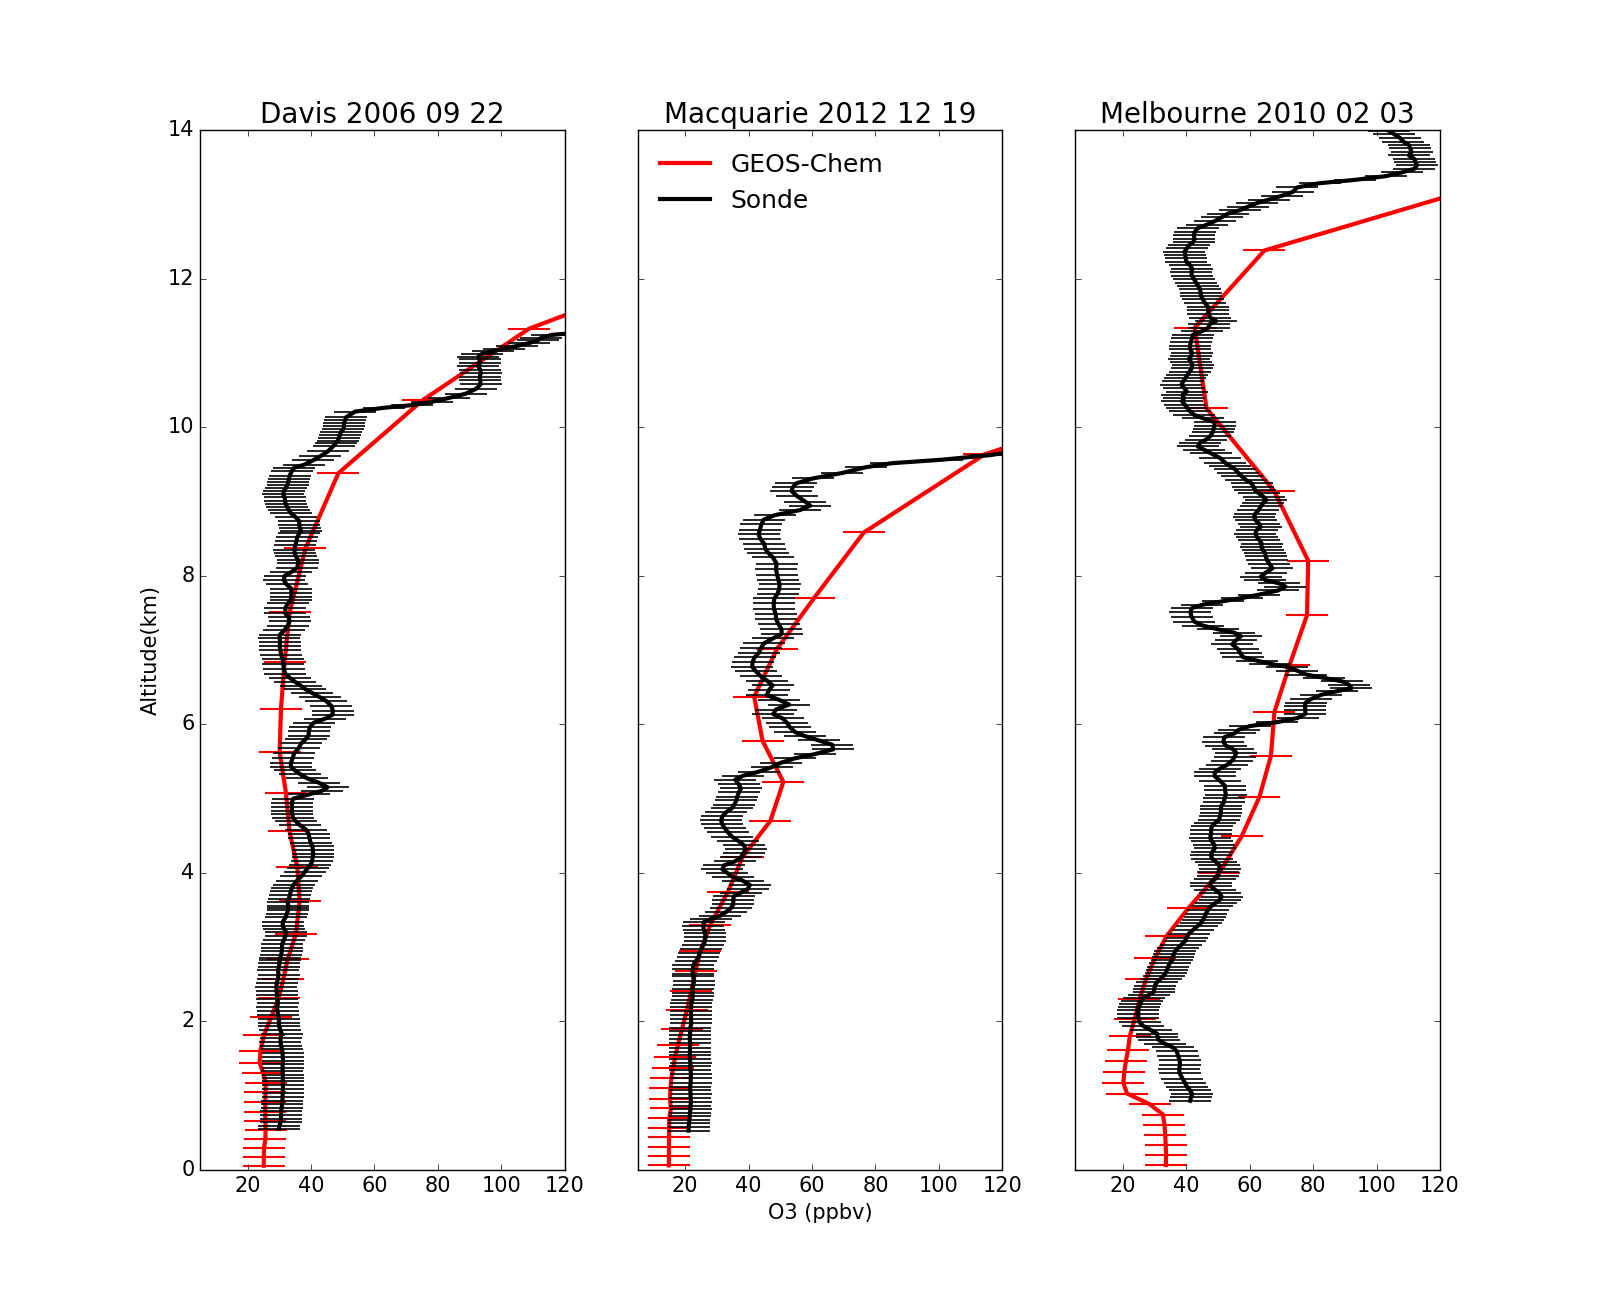
\includegraphics[width=\textwidth]{figures/event_profile_comparison.png}
    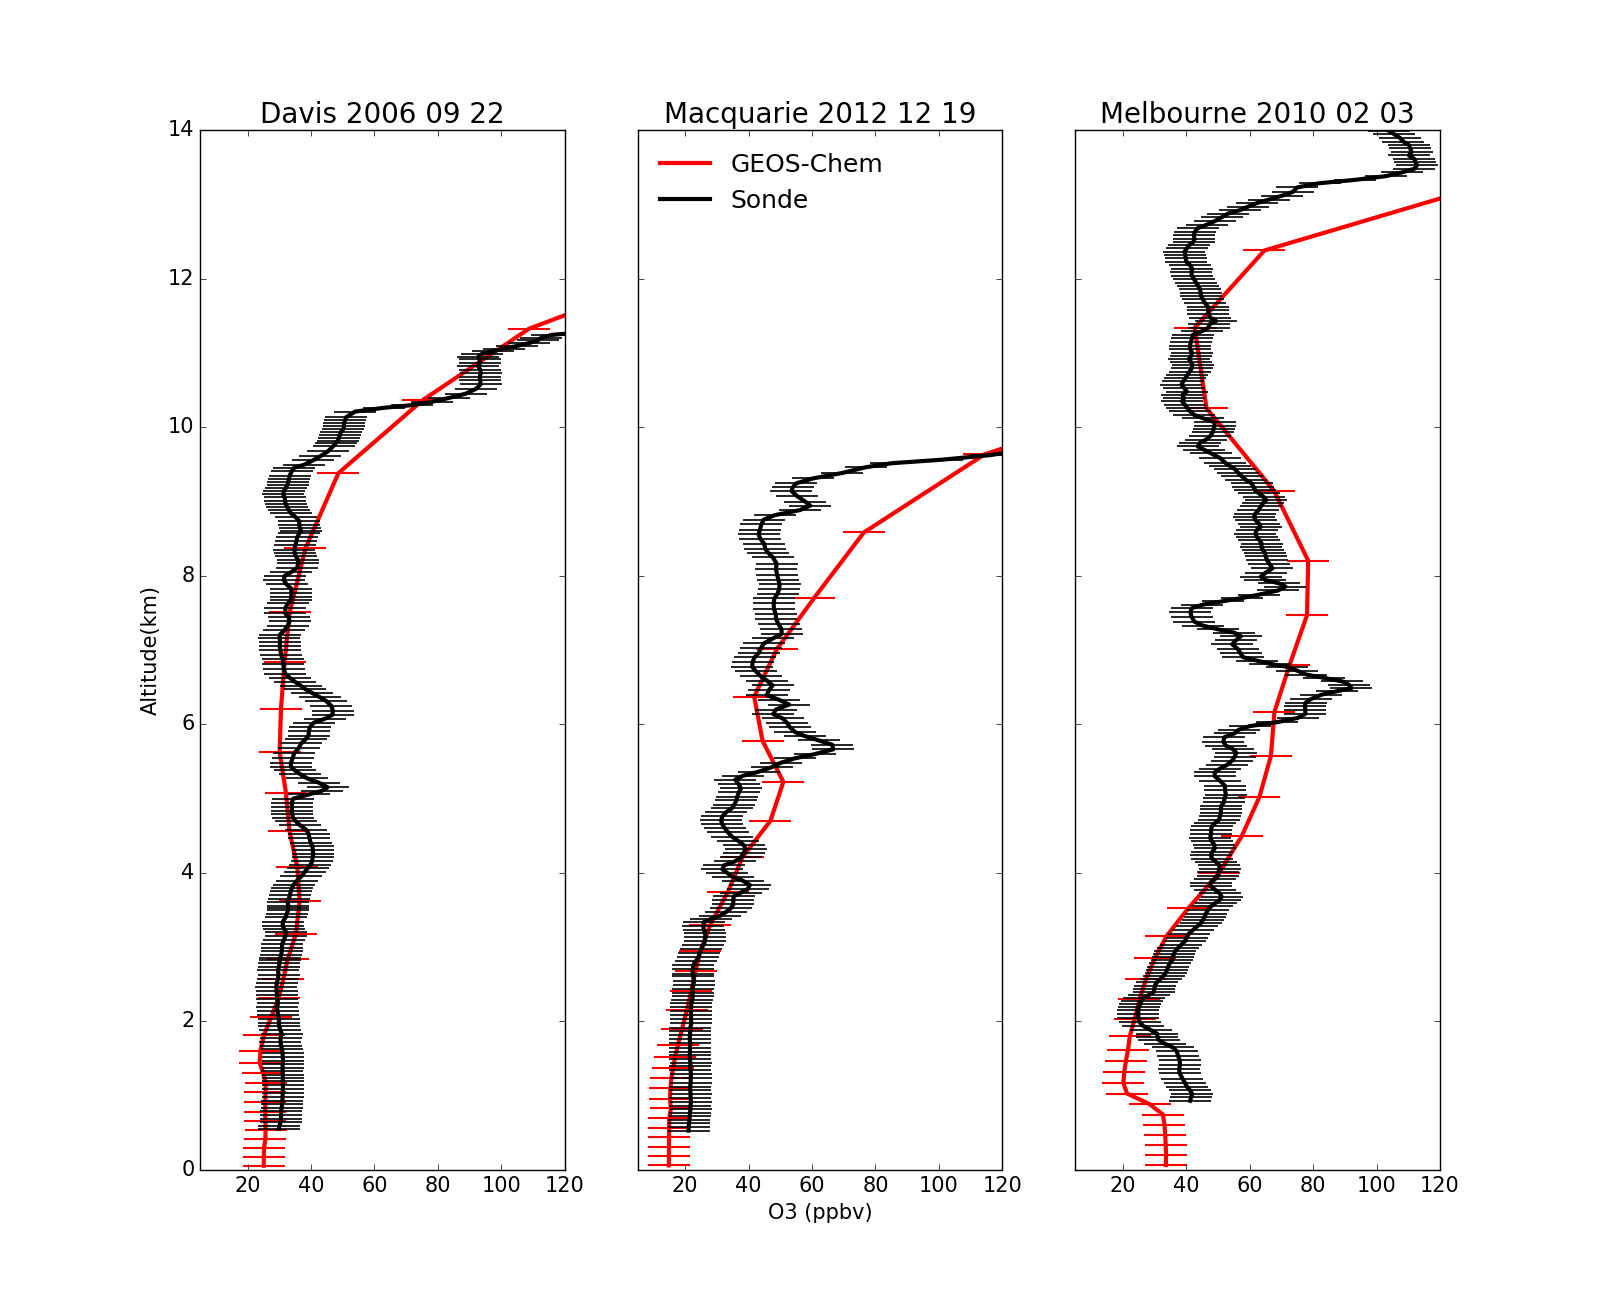
\includegraphics[width=8.3cm]{figures/event_profile_comparison.png}
    \caption{%
      Example comparisons of ozone profiles from ozonesondes (black) and GEOS-Chem (red) from three different dates during which STT events were detected from the measurements.
      The dates were picked based on subjective visual analysis. 
      The examples show the best match between model and observations for each site.
      GEOS-Chem pressure levels are marked with a dash.}
    \label{fig:event_profile_comparison}
  \end{figure}
  
\section{Stratosphere-to-troposphere ozone flux from STT events}
  
  We quantify the mean stratosphere-to-troposphere ozone flux due to STT events at each site based on the integrated ozone amount associated with each STT event (see Sect. \ref{Section:CharacterisationOfSTTs}).
  Events that may have been influenced by transported biomass burning are excluded from this calculation.
  Our estimate provides a conservative lower bound for how much ozone is transported from the stratosphere.
  The estimate is conservative for two main reasons; it ignores secondary ozone peaks which may also be transported from the stratosphere; and it ignores potential ozone enhancements which may have dispersed and increased the local background mixing ratio.
  
  Figure \ref{fig:fluxsummary} shows the mean fraction of total tropospheric column ozone (calculated from ozonesonde profiles) attributed to stratospheric ozone intrusions at each site, averaged over days when an STT event occurred.
  At all sites, the mean fraction of tropospheric ozone attributed to STT events is 2--4\%. On individual days at Macquarie and Melbourne, this value can exceed 10\% .
  Figure \ref{fig:fluxsummaryabs} shows the STT-induced ozone flux in absolute terms.
  We find that the mean ozone flux associated with STT events is $1$-$2 \times 10^{16}$~molecules cm$^{-2}$.
  Our flux estimates are relatively insensitive to our biomass burning filter: including smoke-influenced days changed the mean flux by less than 5\% relative to the absolute values.
  
  \begin{figure}[t]
    \begin{center}
    %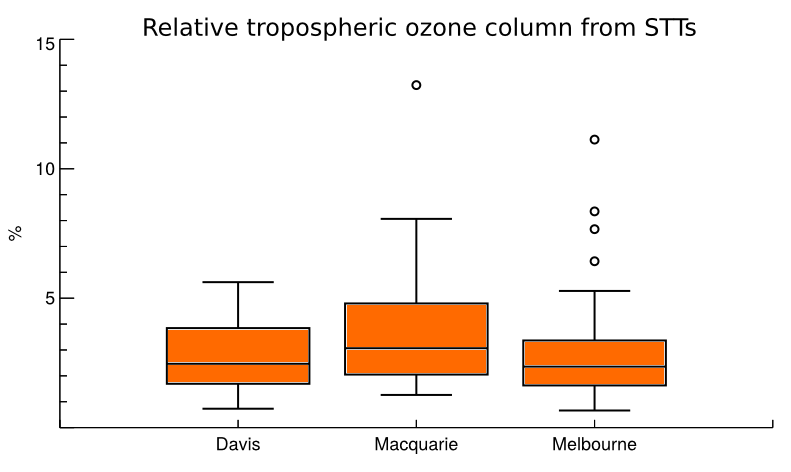
\includegraphics[width=0.8\columnwidth]{figures/flux_relative.png}
    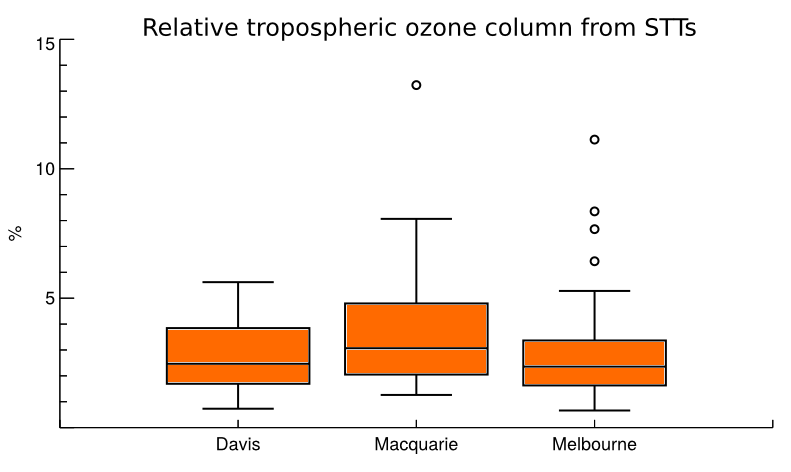
\includegraphics[width=8.3cm]{figures/flux_relative.png}
    \caption{Percent of total tropospheric column ozone attributed to STT events, derived from ozonesonde measurements as described in the text.}
    \label{fig:fluxsummary}
    \end{center}
  \end{figure}
  
  \begin{figure}[t]
  % Flux box and whisker plots from flux_summary.pro in OzoneWork(HPC) and edited in Inkscape
    
    %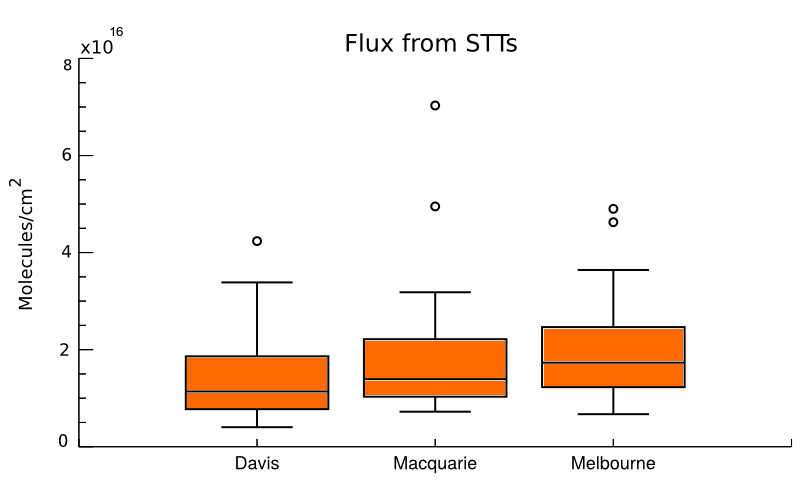
\includegraphics[width=0.8\columnwidth]{figures/flux_absolute.png}
    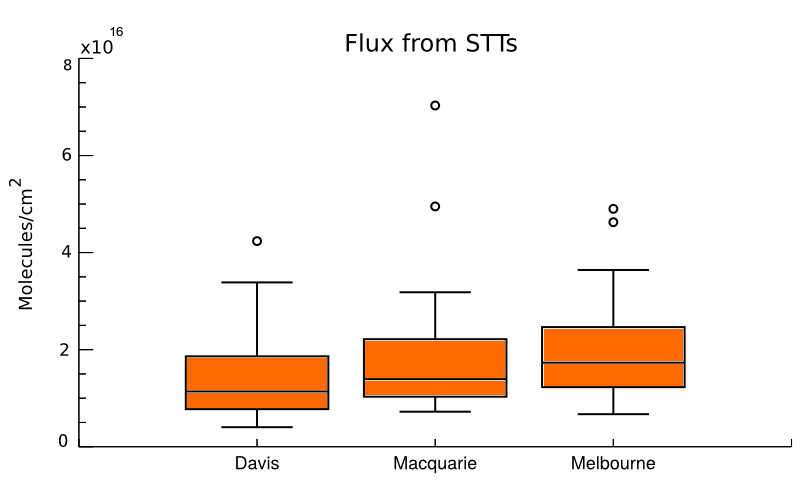
\includegraphics[width=8.3cm]{figures/flux_absolute.png}
    \caption{Tropospheric ozone attributed to STT events, derived from ozonesonde measurements as described in the text.
      Box shows the interquartile range (IQR), with the centre line being the median, whiskers show the minimum and maximum, circles show values which lie more than 1.5 IQR from the median.}
    \label{fig:fluxsummaryabs}
    
  \end{figure}
  
  We use simulated tropospheric ozone columns from GEOS-Chem to extrapolate the ozonesonde-based estimates to the entire Southern Ocean region. 
  To do so, we multiply the monthly likelihoods of STTs (fraction of ozonesonde releases for which an STT event was detected, per month, \textit{f}) by the monthly mean tropospheric ozone column over the Southern Ocean (from the GEOS-Chem multi-year mean, $\Omega_{SO_{O_3}}$) and by the monthly mean fraction of the ozone column attributed to STT \textit{I} (as in Fig. \ref{fig:fluxsummary}).
  The monthly values of each term in this equation are shown in Figure \ref{fig:SOExtrapolation} (lower panel).
  The equation can be written simply as Flux$= \Omega_{SO_{O_3}} \times f \times I$.

  Flux estimation over the southern ocean is based on the average GEOS-Chem tropospheric vertical column of ozone over a particular latitude range.
  The range is from 35$^{\circ}$ S to 75$^{\circ}$ S, chosen to capture the three measurement stations.
  Changing this latitude range by 5$^{\circ}$ in either direction at either end of the range changes the average simulated tropospheric ozone by -7 to 9\%.
  A more spatially resolved estimate could be calculated, by splitting the southern ocean into longitudinal and latitudinal bins.
  This could include using the gradient of flux and frequency estimations along their latitudes, as well as estimated longitudinal variations due to seasonal stratospheric wind jetstreams \citep{Baray2012}.
  An improved spatial distribution for the flux estimation is beyond the scope of this work and would not address the limitations of the estimate shown here.
  
  Figure \ref{fig:SOExtrapolation} (top) shows the extrapolated monthly mean ozone flux from STT events over the Southern Ocean.
  We find from this estimate that STT events may be responsible for at least $3.1 \times10^{16}$~molecules cm$^{-2}$ yr$^{-1}$ of the tropospheric ozone over the Southern Ocean, equivalent to 2.48~Tg yr$^{-1}$.
  %This is calculated using the surface area from GEOS-Chem over the southern ocean grid boxes along with the molecules cm$^{-2}$ per month calculations, along with ozone molar mass of 48~g mol$^{-1}$.
    
  \begin{figure*}[t]
    % Plot from examine_stations.py in stations repo
    %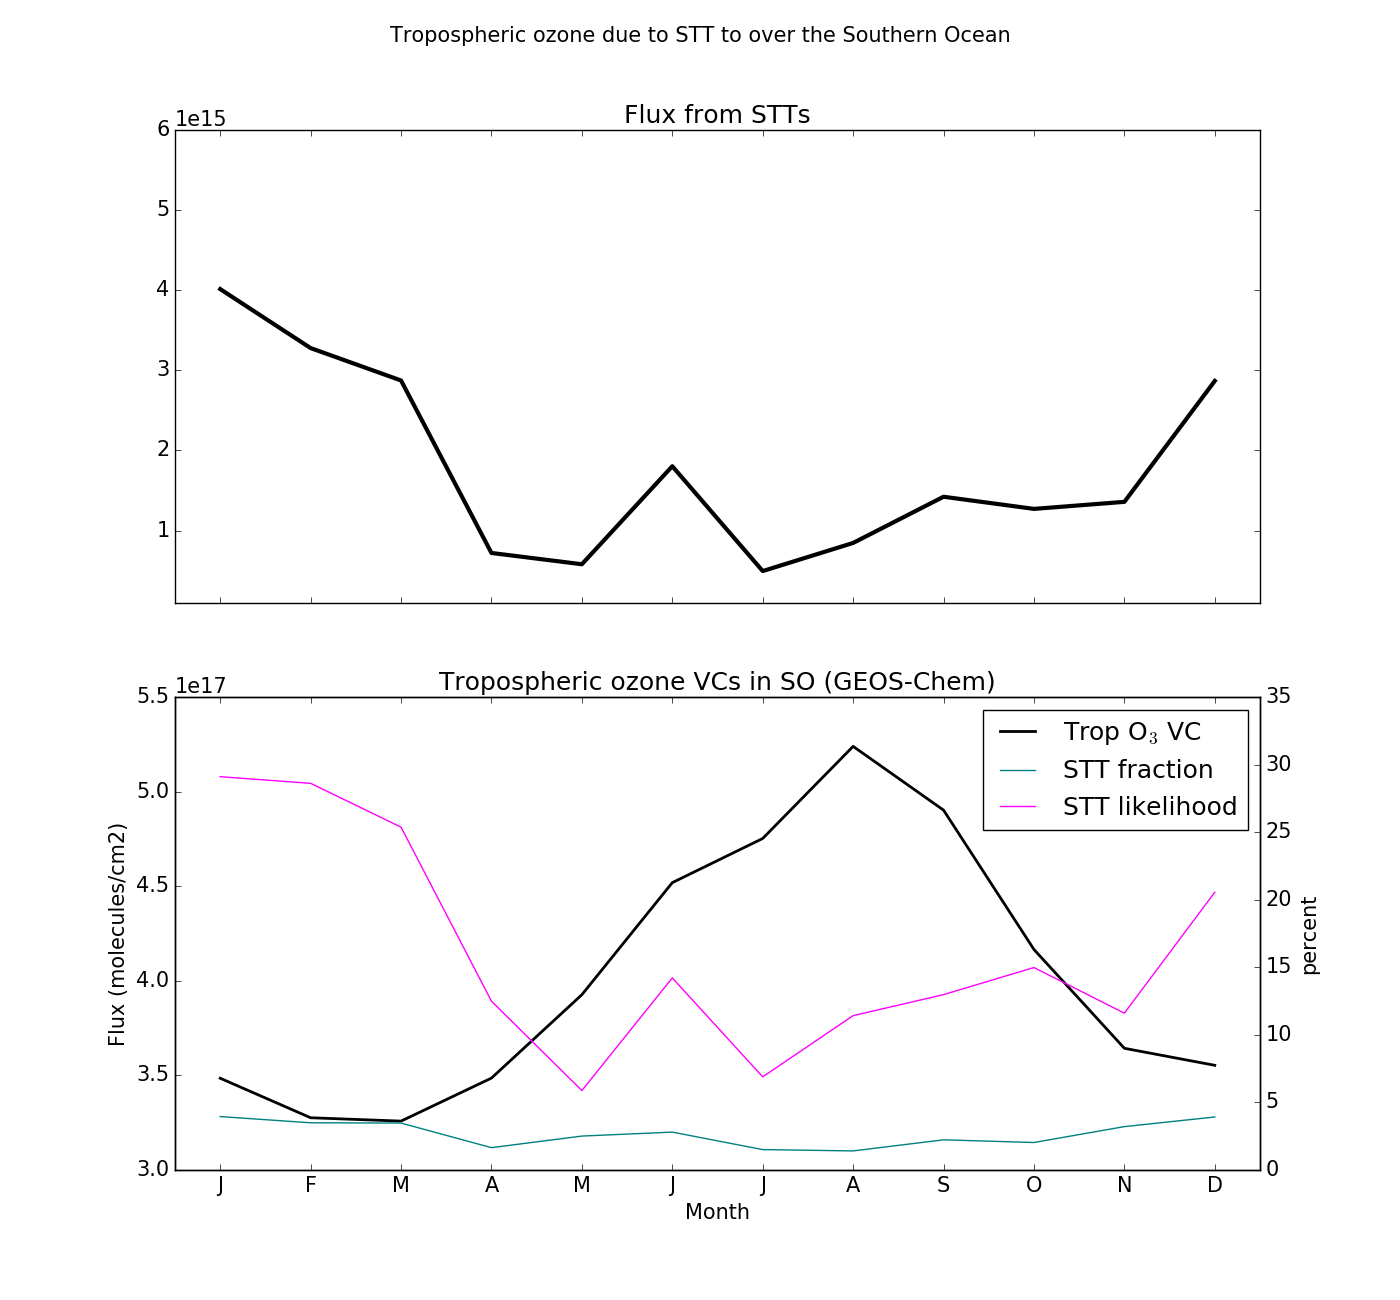
\includegraphics[width=\textwidth]{figures/SO_extrapolation.png}
    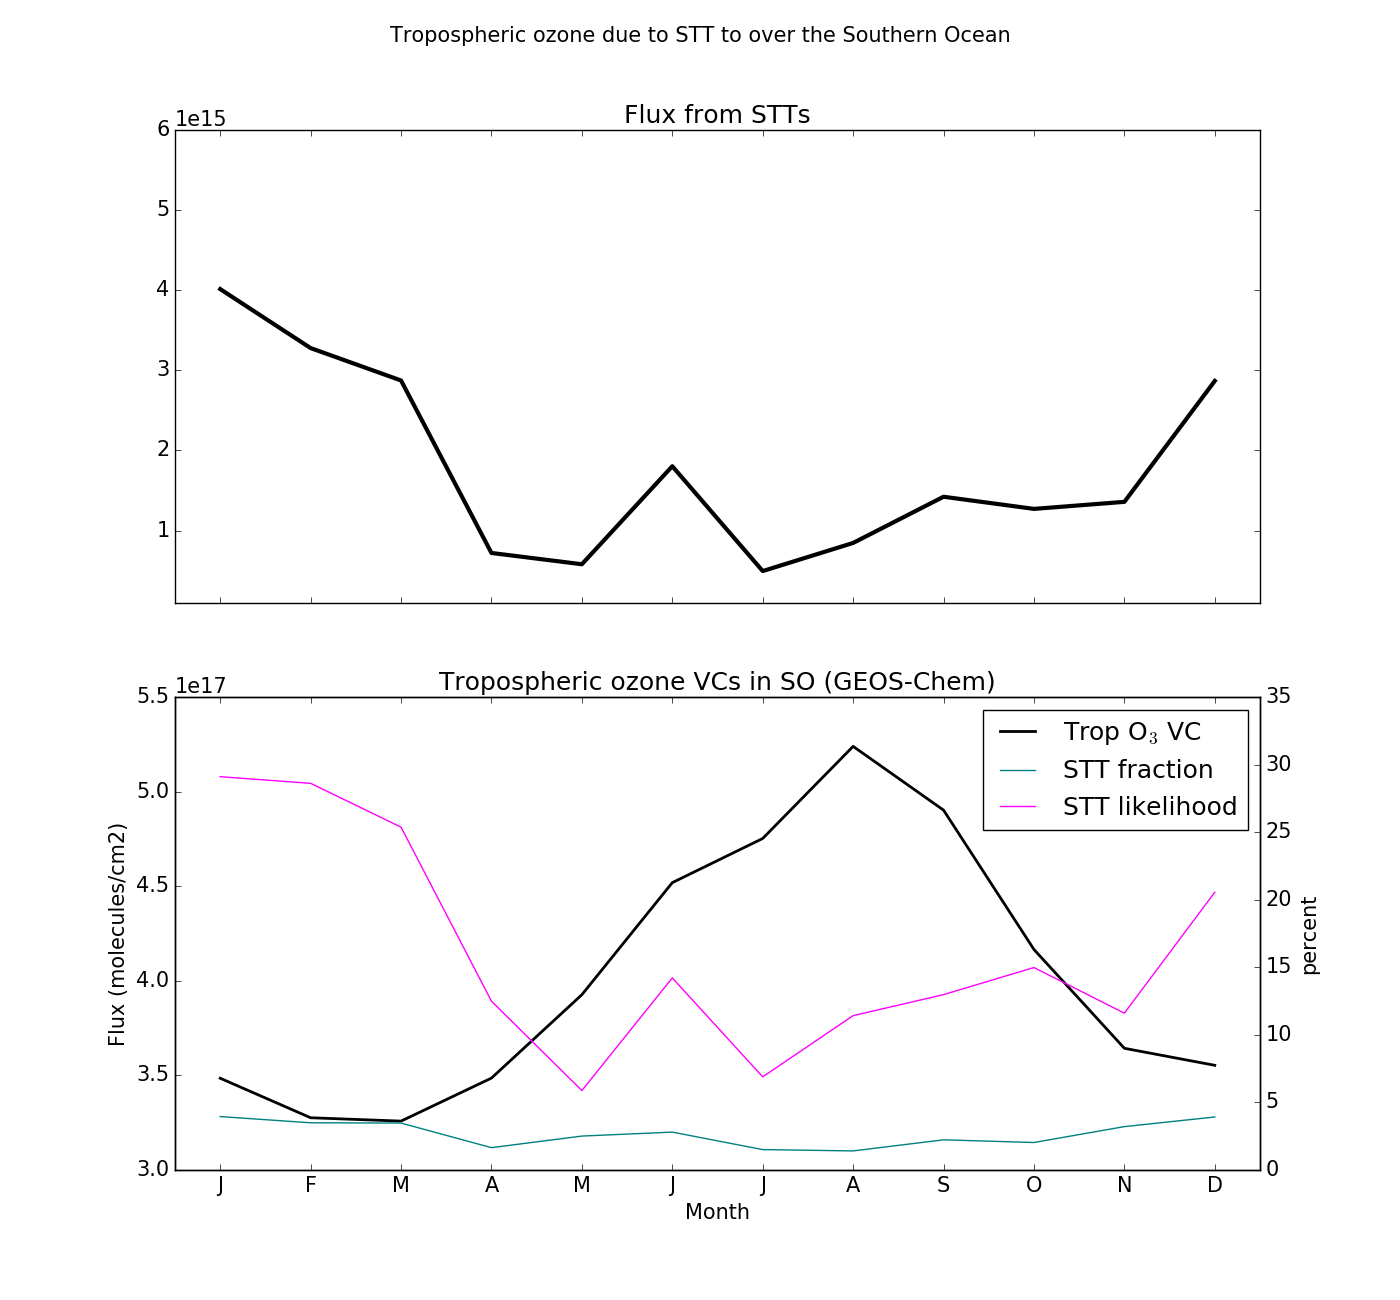
\includegraphics[width=12.0cm]{figures/SO_extrapolation.png}
    \caption{(Top) Estimated contribution of STT to tropospheric ozone columns over the Southern Ocean.
      (Bottom) The three quantities used to calculate (as per the text) the flux estimates shown in the top panel.
      The tropospheric ozone column $\Omega_{SO_{O_3}}$ (black, left axis) is from GEOS-Chem, while the STT $f$raction (blue, right axis) and $I$mpact (purple, right axis) are from the ozonesonde measurements.
      The STT fraction is multiplied by 3 to show the seasonality.}
    \label{fig:SOExtrapolation}
  \end{figure*}
  
  Our estimate is less than other estimates of STT flux, due to our conservative estimate of flux within each event, as well as filtering out events which are too close to the tropopause.
  %Global STT flux estimated from an ensemble of models suggests values around 550~Tg yr$^{-1}$ \citep{Stevenson2006}.
  %Global net downward STT flux is estimated to be 75~Tg yr$^{-1}$ \citep{Sprenger2003}.
  Previous studies have derived global gross STT fluxes of 550~Tg yr$^{-1}$ \citep{Stevenson2006} and net downward STT fluxes of 75~Tg yr$^{-1}$ \citep{Sprenger2003}.
  Our estimate of 2.48~Tg yr$^{-1}$ would suggest only $\sim$3.3\% of the global net downward flux can be attributed to STT events in the southern ocean, a value that is likely too low.
  %This method of flux estimation could be increased if we could account for background ozone enhancement and mixing due to events.
  This result highlights one of the difficulties associated with temporally sparse ozonesonde data, as STT impact is hard to measure without multiple measurements during and surrounding an event.
  
  %It's also worth noting that our flux estimate only detects STT events that satisfy specific criteria, and may therefore be unsuitable for calculating more general STT fluxes.
  
  %\citet{Olsen2003} used PV and winds from the GEOS reanalysis combined with ozone measurements from the TOMS satellite to estimate that the ozone flux between 30$^{\circ}$ S and 60$^{\circ}$ S 210~Tg yr$^{-1}$ .
  %Their estimates show peak ozone flux from winter to early spring (JJAS).
  %\citet{Liu2016} model the upper tropospheric ozone and it's source (emissions/lightning/stratospheric) over the Atlantic ocean between 30$^{\circ}$ S and 45$^{\circ}$ S, and suggest that most of this is transported from the stratosphere from March to September, which is when the subtropical jet system is strongest.
  Other studies have found increased STT ozone fluxes in the SH extratropics occur from autumn or winter to early spring \citep{Olsen2003, Liu2016}. 
  At this time of year, we find the highest tropospheric $\Omega_{O3}$, but a relatively low STT flux.
  Our results suggest instead that the ozone flux associated with STT events (at least those due to tropopause folds) is largest in austral summer (December-March), primarily due to an increased frequency of STT detections during these months.
  Some legitimate STT events may have been removed due to coincident smoke plumes, which could affect our STT event frequency during winter.
  %It is worth noting that the 30$^{\circ}$ S to 60$^{\circ}$ S latitudes describe the Ferrel cell, while our region of analysis also includes some of the Polar cell.

  %Considering the individual event contributions, \citet{Terao2008} estimate much higher STT impacts using a global CTM with a stratospheric ozone tracer; where 30--40\% of the 500~hPa ozone is due to STT.
  As described previously, our estimate of the fraction of tropospheric ozone from each STT event ($I$) is almost certainly biased low, perhaps by a significant amount. 
  Using a global CTM with a stratospheric ozone tracer, \citet{Terao2008} estimated that this number was closer to 30--40\%, at least for the ozone mixing ratio at 500~hPa in the northern hemisphere.
  %Although this figure is based on the Northern Hemisphere upper troposphere, if we assume that STT flux due to an event is actually 35\% (instead of using our estimated influence) our estimate increases by roughly a factor of 12: to $\sim$30.2~Tg yr$^{-1}$
  If we we assume a fractional ozone flux due to each event STT event of $f$=35\% based on their results (rather than our calculation of 2-4\%), our estimate of the net downward ozone STT flux from southern ocean STT events increases by an order of magnitude to $\sim$29.5~Tg yr$^{-1}$ which is 39\% of the global net downward flux estimated by \citet{Sprenger2003}.

%  This would suggest that tropopause fold ozone transport events over the southern ocean account $\sim$40.3\% of global net STT flux.
  
